\chapter{Basic Min-plus and Max-plus Calculus}
\label{L10}
%  Rasssembler dans un chapitre tout ce qui est theorie, pour un acces
%   rapide au lecteur presse. Eviter de faire un chapitre indigeste
%   qui rende le livre inaccessible au lecteur presse. Pour cela,
%   faire deux parties: resultats de base, resultats avances
%\section{Introduction}
In this chapter we introduce the basic results from Min-plus that
are needed for the next chapters. Max-plus algebra is dual to
Min-plus algebra, with  similar concepts and results when minimum
is replaced by maximum, and infimum by supremum. As basic results
of network calculus use more min-plus algebra than max-plus
algebra, we present here in detail the fundamentals of min-plus
calculus. We briefly discuss the care that should be used when max
and min operations are mixed at the end of the chapter. A detailed
treatment of Min- and Max-plus algebra is provided in
\cite{maxPlus}, here we focus on the basic results that are needed
for the remaining of the book. Many of the results below can also
be found in \cite{Changbook} for the discrete-time setting.
\section{Min-plus Calculus}
\mylabel{sec:minplus}
%Let $\calS$ be a nonempty subset of $\Reals$.
In conventional algebra, the two most common operations on
elements of $\Ints$ or $\Reals$ are their addition and their
multiplication. In fact, the set of integers or reals endowed with
these two operations verify a number of well known axioms that
define algebraic structures: $(\Ints, +, \times)$  is a
commutative ring, whereas $(\Reals, +, \times)$ is a field.
 Here we consider another algebra, where the operations are changed as follows:
addition becomes computation of the minimum,
multiplication becomes addition. We will see that this defines another algebraic structure,
but let us first recall the notion of minimum and infimum.

%Let $\calS$ be a nonempty subset of $\Reals$. $\calS$ is bounded from above (respectively below)
%if there is a number~$M$ such that $s \leq M$ (resp. $s \geq M$) for all $s \in \calS$. The completeness
%axiom states that every nonempty subset $S$  of $\Reals$ that is bounded from above (resp. below)
%has a least upper bound (resp. greatest lower bound).
%We will call it {\em supremum} (resp. {\em infimum}) of~$\calS$, and
% denote it by $\sup \calS$ (resp. $\inf \calS$).
\subsection{Infimum and Minimum}
\mylabel{sec:infmin}
\index{minimum}
\index{infimum}
\index{1wedge@$\wedge$ (min or inf)}
Let $\calS$ be a nonempty subset of $\Reals$.
$\calS$ is bounded from below if there is a number~$M$ such that
$s \geq M$ for all $s \in \calS$. The completeness axiom states
that every nonempty subset $\calS$  of $\Reals$ that is bounded
from below has a greatest lower bound. We will call it {\em
infimum} of~$\calS$, and denote it by $\inf \calS$. For example
the closed and open intervals $[a,b]$ and $(a,b)$ have the same
infimum, which is $a$. Now, if $\calS$ contains an element that is
smaller than all its other elements, this element is called
  {\em minimum} of~$\calS$, and is denoted by $\min \calS$. Note that the minimum of a set does not always
exist. For example, $(a,b)$ has no minimum since $a \notin  (a,b)$. On the other hand, if the
minimum of a set $\calS$ exists, it is identical to its infimum. For example, $\min [a,b] = \inf [a,b] = a$.
One easily shows that every finite nonempty subset of $\Reals$ has a minimum.
Finally, let us mention that we will often use the notation $\wedge$ to denote infimum (or, when it
exists, the minimum). For example, $a \wedge b = \min \{ a, b \}$.
If  $\calS$ is empty, we adopt the convention that $\inf \calS = +\infty$.

If $f$ is a function from $\calS$ to $\Reals$, we denote by $f(\calS)$ its range:
$$ f(\calS) = \{ t \mst t = f(s) \; \mbox{ for some } s \in \calS \}. $$
We will denote the infimum of this set by the two equivalent notations
$$ \inf f(\calS) = \inf_{s \in \calS} \{ f(s) \}. $$
We will also often use the following property.
\begin{theorem}[``Fubini'' formula for infimum]
\mylabel{thm:fubini}
Let $\calS$ be a nonempty subset of $\Reals$, and $f$ be a function from $\calS$ to $\Reals$.
Let $\{ \calS_n \}_{n \in \Nats}$ be a collection of subsets of $\calS$, whose union is $\calS$. Then
$$ \inf_{s \in \calS} \{ f(s) \} = \inf_{n \in \Nats} \left\{ \inf_{s \in \calS_n} \{ f(s_n) \} \right\} . $$
\end{theorem}
\pr By definition of an infimum, for any sets $\calS_n $,
$$ \inf \left\{ \bigcup_{n} \calS_n \right\} = \inf_{n} \left\{ \inf  \calS_n \right\}.$$
On the other hands, since $\cup_{n} \calS_n = \calS$,
$$ f \left( \bigcup_{n \in \Nats} \calS_n \right) = \bigcup_{n \in \Nats} f \left( \calS_n \right) $$
so that
\begin{eqnarray*}
\inf_{s \in \calS} \{ f(s) \} & = & \inf  f(\calS) =  \inf  f \left( \bigcup_{n \in \Nats} \calS_n \right) \\
& = &  \inf \left\{ \bigcup_{n \in \Nats} f \left( \calS_n \right) \right\} =
\inf_{n \in \Nats} \left\{ \inf f \left(  \calS_n \right) \right\} \\
& = & \inf_{n \in \Nats} \left\{ \inf_{s \in \calS_n} \{ f(s) \} \right\} .
\end{eqnarray*}
\qed
\subsection{Dioid $( \Reals \cup \{ +\infty \}, \wedge, +)$}
\mylabel{sec:dioid}
\index{dioid}
In traditional algebra, one is used to working with the algebraic
structure $( \Reals, + , \times )$, that is, with the set of reals
endowed with the two usual operations of addition and
multiplication. These two operations possess a number of
properties (associativity, commutativity, distributivity, etc)
that make $( \Reals, + , \times )$ a commutative field. As
mentioned above, in min-plus algebra, the operation of `addition'
becomes computation of the infimum (or of the minimum if it
exists), whereas the one of `multiplication' becomes the classical
operation of addition. We will also include $ +\infty $ in the set
of elements on which min-operations are carried out, so that the
structure of interest is now  $(\Reals \cup  \{ +\infty \},
\wedge, +)$. Most axioms (but not all, as we will see later)
defining a field still apply to this structure. For example,
distribution of addition with respect to multiplication in
conventional (`Plus-times') algebra
$$ (3 + 4) \times 5  = (3 \times 5) + (4 \times 5) = 15 + 20 = 35 $$
%
%\begin{eqnarray*}
%(3 \times 4) + (2 \times 5) & = & 22 \\
%(3 + 4) \times 5  = & 49
%\end{eqnarray*}
%
translates in min-plus algebra as
$$ (3 \wedge 4) + 5  = (3 + 5) \wedge (4 + 5) = 8 \wedge 9 = 8. $$
%\begin{eqnarray*}
%(3 + 4) \wedge (2 + 5) & = & 7 \\
%(3 \wedge 4) + (2 \wedge 5) & = & 5
%\end{eqnarray*}
In fact, one easily verifies that $\wedge$ and $+$ satisfy the following properties:
%
%, which is here the operation of `addition',
%verifies the following properties:
\begin{itemize}
\item{ \textbf{(Closure of $\wedge$)} For all $a, b  \in \Reals \cup \{ +\infty \}$,
$a \wedge b \in \Reals \cup \{ +\infty \}$.}
\item{ \textbf{(Associativity of $\wedge$)} For all $a, b, c \in \Reals \cup \{ +\infty \}$,
$(a \wedge b) \wedge c =  a \wedge (b \wedge c)$.}
\item{ \textbf{(Existence of a zero element for $\wedge$)}
There is some $\mbox{e} = +\infty \in \Reals \cup \{ +\infty \}$
such that for all $a \in \Reals \cup \{ +\infty \}$, $a \wedge
\mbox{e} = a$.}
\item{ \textbf{(Idempotency of $\wedge$)}  For all $a  \in \Reals \cup \{ +\infty \}$,
$a \wedge a = a$.}
\item{ \textbf{(Commutativity of $\wedge$)} For all $a, b \in \Reals \cup \{ +\infty \}$,
$a \wedge b = b \wedge a$.}
%\end{itemize}
%The operation $+$, which is here the operation of `multiplication', has the following properties
%\begin{itemize}
\item{ \textbf{(Closure of $+$)} For all $a, b  \in \Reals \cup \{ +\infty \}$,
$a + b \in \Reals \cup \{ +\infty \}$.}
\item{ \textbf{(Associativity of $+$)} For all $a, b, c \in \Reals \cup \{ +\infty \}$,
$(a + b) + c =  a + (b + c)$.}
\item{ \textbf{(The zero element for $\wedge$ is absorbing for $+$)}
For all $a \in \Reals \cup \{ +\infty \}$, $a + \mbox{e} =  \mbox{e} =  \mbox{e}+ a$.}
\item{ \textbf{(Existence of a neutral element for $+$)}
There is some $u = 0 \in \Reals \cup \{ +\infty \}$ such that for
all $a \in \Reals \cup \{ +\infty \}$, $a + u = a = u + a$.}
%\item{ \textbf{(Commutativity of $+$)} For all $a, b \in \Reals \cup \{ +\infty \}$,
%$a + b =  b + a$.}
%\end{itemize}
%Finally, $+$ is distributive with respect to $\wedge$:
\item{ \textbf{(Distributivity of $+$ with respect to $\wedge$)} For all $a, b, c  \in \Reals \cup \{ +\infty \}$,
$(a \wedge b) + c =  (a + c) \wedge (b + c) = c + (a \wedge b)$. }
\end{itemize}
A set endowed with operations satisfying all the above axioms is called a {\em dioid}.
Moreover as $+$ is also commutative (for all $a, b \in \Reals \cup \{ +\infty \}$,
$a + b =  b + a$), the structure $(\Reals \cup  \{ +\infty \}, \wedge, +)$ is a commutative dioid.
%The structure $(\Reals \cup  \{ +\infty \}, \wedge , +)$ is not a field any more, because
%one axiom is no longer valid.
All the axioms defining a dioid are therefore the same axioms as
the ones defining a ring, except one: the axiom of idempotency of
the `addition', which in dioids replaces the axiom of cancellation
of `addition' in rings (i.e. the existence of an element $(-a)$
that `added' to $a$ gives the zero element). We will encounter
other dioids later on in this chapter.
\subsection{A Catalog of Wide-sense Increasing Functions}
\mylabel{sec:wsifunctions}
\index{1calG@$\calG$ (set of wide-sense increasing functions)}
\index{1calF@$\calF$ (set of wide-sense increasing functions that
are zero for negative arguments)}
A function $f$ is wide-sense increasing if and only if $f(s) \leq
f(t)$ for all $s \leq t$. We will denote by $\calG$ the set of
non-negative wide-sense increasing sequences or functions and by
$\calF$ denote the set of  wide-sense increasing sequences or
functions such that $f(t) = 0$ for $t < 0$. Parameter $t$ can be
continuous or discrete: in the latter case, $f = \{ f(t), t \in
\Ints \}$ is called a sequence rather than a function. In the
former case, we take the convention that the function $f = \{
f(t), t \in \Reals \}$ is left-continuous. The range of functions
or sequences of $\calF$ and $\calG$ is $\Reals^{+} = [0,+\infty]
$.

%Clearly, $\calF \subseteq \calG$.
Notation $f + g$ (respectively $f \wedge g$) denotes the point-wise sum (resp. minimum) of
functions $f$ and $g$:
\begin{eqnarray*}
(f + g)(t) & = & f(t) + g(t) \\
(f \wedge g)(t) & = & f(t) \wedge g(t)
\end{eqnarray*}
Notation $f \leq (=, \geq) g$ means that $f(t) \leq (=, \geq) g(t)$ for all $t$.

Some examples of functions belonging to $\calF$ and of particular interest are the
following ones.
Notation $[x]^{+}$ denotes $\max \{x,0 \}$,  $\lceil x \rceil$ denotes the smallest integer larger than or equal to $x$.
\index{1lambda@$\lambda_{R}$ (peak rate function)}
\index{peak rate function}
\begin{definition}[Peak rate functions $\lambda_{R}$]
\mylabel{def:peakrate}
$$
\lambda_{R}(t)= \left\{ \begin{array}{ll}  Rt & \mbox{ if } t > 0 \\
                        0 & \mbox{ otherwise }
\end{array}
\right.
$$
for some $R \geq 0$ (the `rate').
\end{definition}
\index{1delta@$\delta_{T}$ (burst delay function)}
\index{burst delay function}
\begin{definition}[Burst delay functions $\delta_{T}$]
\mylabel{def:burstdelay}
$$
\delta_{T}(t)= \left\{  \begin{array}{ll}  +\infty & \mbox{ if } t > T \\
                        0 & \mbox{ otherwise }
\end{array}
\right.
$$
for some $T \geq 0$ (the `delay').
\end{definition}
\index{1beta@$\beta_{R,T}$ (rate-latency function)}
\index{rate-latency function}
\begin{definition}[Rate-latency functions $\beta_{R,T}$]
\mylabel{def:ratelatency}
$$
\beta_{R,T}(t) = R [t-T]^{+} = \left\{  \begin{array}{ll}  R(t-T) & \mbox{ if } t > T \\
                        0 & \mbox{ otherwise }
\end{array}
\right.
$$
for some $R \geq 0$ (the `rate') and $T \geq 0$ (the `delay').
\end{definition}
\index{1gamma@$\gamma_{r,b}$ (affine function)}
\index{affine function}
\begin{definition}[Affine functions $\gamma_{r,b}$]
\mylabel{def:affine}
$$ \gamma_{r,b}(t) = \left\{ \begin{array}{ll} rt + b & \mbox{ if } t > 0 \\
                    0 & \mbox{ otherwise }
\end{array}
\right.
$$
for some $r \geq 0$ (the `rate') and $ b \geq 0$ (the `burst').
\end{definition}
\index{1u@$v_{T}$ (step function)}%
\index{step function}%
\begin{definition}[Step Function $v_{T}$]
\mylabel{def:stepfunction}
$$ v_{T}(t) = 1_{ \{ t > T \} } = \left\{ \begin{array}{ll} 1 & \mbox{ if } t > T \\
                    0 & \mbox{ otherwise }
\end{array}
\right.
$$
for some $T > 0$.
\end{definition}
\index{1u@$u_{T, \tau}$ (staircase function)}%
\index{staircase function}%
\begin{definition}[Staircase Functions $u_{T,\tau}$]
\mylabel{def:staircase}
\mylabel{step}
$$ u_{T, \tau}(t) = \left\{ \begin{array}{ll} \lceil \frac{t+ \tau}{T} \rceil & \mbox{ if } t > 0 \\
                    0 & \mbox{ otherwise }
\end{array}
\right.
$$
for some $T > 0$ (the `interval') and $ 0 \leq \tau \leq T$ (the `tolerance').
\end{definition}

These functions are also represented in Figure~\ref{fig:examplesoffunctions}.
\begin{figure}[!htbp]
   \insfig{Examplesoffunctions}{0.7}
  \mycaption{A catalog of functions of $\calF$: Peak rate function (top left), burst-delay function (top right),
rate-latency function (center left), affine function (center right), staircase function (bottom left) and step function (bottom right).}
  \mylabel{fig:examplesoffunctions}
\end{figure}
By combining these basic functions, one obtains more general piecewise linear functions belonging
to $\calF$. For example, the two functions represented in Figure~\ref{fig:examplesofpwlfunctions}
are written using $\wedge$ and $+$ from affine functions and rate-latency functions as follows,
with $r_1 > r_2 > \ldots > r_I$ and $b_1 < b_2 < \ldots < b_I$
\begin{eqnarray}
\mylabel{eq:pwlconcave}
f_1 & = & \gamma_{r_1,b_1} \wedge  \gamma_{r_2,b_2} \wedge \ldots \gamma_{r_I,b_I} % \nonumber  \\
   =   \min_{1 \leq i \leq I} \{ \gamma_{r_i,b_i} \} \\
%   =   \bigwedge_{i=1}^{I} \gamma_{r_i,b_i} \\
\mylabel{eq:pwlsubadditive} f_2 & = & \lambda_R \wedge \{
\beta_{R,2T} + RT \} \wedge  \{ \beta_{R,4T} + 2RT\} \wedge \ldots
\nonumber \\
    & = &  \inf_{i \geq 0} \left\{  \beta_{R,2iT} + iRT \right\}.
%     =  \bigwedge_{i \geq 0} \left\{  \beta_{R,iT} + iRT \right\}.
    %  & = & \bigwedge_{i \geq 0} \left\{ R[t-iT]^{+} + iRT \right\}
\end{eqnarray}
\begin{figure}[!htbp]
   \insfig{Examplesofpwlfunctions}{0.8}
  \mycaption{Two piecewise linear functions of $\calF$ as defined by (\ref{eq:pwlconcave}) (left) and
(\ref{eq:pwlsubadditive}) (right).}
  \mylabel{fig:examplesofpwlfunctions}
\end{figure}
We will encounter other functions later in the book, and obtain
other representations with the min-plus convolution operator.
\subsection{Pseudo-inverse of Wide-sense Increasing Functions}
\mylabel{sec:pseudo-inverse}
It is well known that any strictly increasing function is
left-invertible. That is, if for any $t_1 < t_2$, $f(t_1) <
f(t_2)$, then there is a function $f^{-1}$ such that $f^{-1}(f(t))
= t$ for all $t$. Here we consider slightly more general
functions, namely, wide-sense increasing functions, and we will
see that a pseudo-inverse function can defined as follows.
\index{pseudo-inverse function}
\begin{definition}[Pseudo-inverse]
\mylabel{def:pseudo-inverse}
Let $f$ be a function or a sequence of $\calF$. The pseudo-inverse of $f$ is the function
\begin{equation}
\mylabel{eq:pseudo-inverse}
f^{-1}(x) = \inf \left\{ t  \mst f(t) \geq x \right\}.
\end{equation}
%if this set is nonempty and is $f^{-1}(x) = +\infty$ if this set is empty (that is, when
%$f(t) < x$ for all $t$).
\end{definition}
For example, one can easily compute that the pseudo-inverses of the four functions of Definitions~\ref{def:peakrate} to
\ref{def:affine} are
\begin{eqnarray*}
\lambda_R^{-1} & = & \lambda_{1/R} \\
\delta_{T}^{-1} & = & \delta_0 \wedge T \\
\beta_{R,T}^{-1} & = & \gamma_{1/R,T}\\
\gamma_{r,b}^{-1} & = & \beta_{1/r,b}.
\end{eqnarray*}
The pseudo-inverse enjoys the following properties:
\begin{theorem}[Properties of pseudo-inverse functions]
\mylabel{thm:propertiespseudo-inverse}
Let $f \in \calF$, $x,t \geq 0$.
\begin{itemize}
\item{\textbf{(Closure)}  $f^{-1} \in \calF$ and $f^{-1}(0) = 0$.}
\item{\textbf{(Pseudo-inversion)} %If $f(t) \geq x$ then $ f^{-1}(x) \leq t $.
%Conversely, if $ f^{-1}(x) \geq t $ then $f(t) \leq x$.
We have that
\begin{eqnarray}
\mylabel{eq:pseudo-inverse(i)}
f(t) \geq x & \Rightarrow & f^{-1}(x) \leq t \\
\mylabel{eq:pseudo-inverse(ii)}
f^{-1}(x) < t & \Rightarrow & f(t) \geq x  %\\
%\mylabel{eq:pseudo-inverse(iii)}
%f^{-1}(x) \geq t & \leftdoublearrow & f(t) \leq x \\
%\mylabel{eq:pseudo-inverse(iiii)}
%f(t) < x & \leftdoublearrow & f^{-1}(x) \geq t .
\end{eqnarray}
}
\item{\textbf{(Equivalent definition)}
\begin{equation}
\mylabel{eq:dualpseudo-inverse}
f^{-1}(x) = \sup \left\{ t  \mst f(t) < x \right\}.
\end{equation}
}
%\item{\textbf{(Duality)} One can compute $f$ from $f^{-1}$ by
%\begin{equation}
%\mylabel{eq:dualpseudo-inverse}
%f(t) = \inf \left\{ x  \mst f^{-1}(x) \geq t \right\}.
%\end{equation}
%}
%\item{ \textbf{(Concave and convex functions)} $f^{-1}$ is concave (respectively convex) if and only if
%$f$ is convex (resp. concave).}
\end{itemize}
\end{theorem}
%We prove here the two first properties only (the third one is not used in this book (cancel? exercise?)
\pr Define subset $\calS_{x} = \left\{ t \mst f(t) \geq x \right\}
\subseteq \Reals^{+}$. Then (\ref{eq:pseudo-inverse}) becomes $
f^{-1}(x) = \inf \calS_{x} $. \vspace{1ex} \noindent (Closure)
Clearly, from (\ref{eq:pseudo-inverse}), $f^{-1}(x) = 0$ for $x
\leq 0$ (and in particular $f^{-1}(0) = 0$). Now, let $0 \leq x_1
< x_2 $. Then $\calS_{x_1} \supseteq \calS_{x_2}$, which implies
that $ \inf \calS_{x_1} \leq \inf \calS_{x_2} $ and hence that $
f^{-1}(x_1) \leq  f^{-1}(x_2) $. Therefore $f^{-1}$ is wide-sense
increasing.
\vspace{1ex}
\noindent (Pseudo-inversion) Suppose
first that $f(t) \geq x$. Then  $t \in \calS_{x}$, and so is
larger than the infimum of $\calS_{x}$, which is $f^{-1}(x)$: this
proves (\ref{eq:pseudo-inverse(i)}).
%\noindent
Suppose next that $f^{-1}(x) < t$. Then  $t > \inf \calS_{x}$, which implies that
$t \in \calS_{x}$, by definition of an infimum. This in turn yields that $f(t) \geq x$
and proves (\ref{eq:pseudo-inverse(ii)}).
%
%
%Suppose next that  $f^{-1}(x) \geq t$. As $f$ is wide-sense increasing, it implies that
%$f(f^{-1}(x)) \geq f(t)$. Because of (\ref{eq:pseudo-inverse(i)}),
%We have shown that the latter inequality implies that
%$f^{-1}(x) \geq f^{-1}(f(t))$. As $f^{-1}$ is also wide-sense increasing, it yields that
%$x \geq f(t)$, that is (\ref{pseudo-inverse(ii)})
%
%Finally, suppose that $f(t) < x$. Then
 %as $f^{-1}$ is wide-sense increasing,
%$f^{-1}(f(t)) \geq f^{-1}(x)$.
%
\vspace{1ex}
\noindent
(Equivalent definition) Define subset $\tilde{\calS}_{x} = \left\{ t \mst f(t) < x \right\} \subseteq \Reals^{+}$. Pick $t \in \calS_x$ and $\tilde{t} \in \tilde{\calS}_{x}$. Then $f(\tilde{t}) < f(t)$, and since $f$ is wide-sense increasing, it implies that $\tilde{t} \leq t$. This is true for any  $t \in \calS_x$ and $\tilde{t} \in \tilde{\calS}_{x}$, hence $\sup \tilde{\calS}_{x} \leq \inf \calS_{x} $. As $\tilde{\calS}_{x} \cup \calS_{x} = \Reals^{+}$, we cannot have $\sup \tilde{\calS}_{x} < \inf \calS_{x} $. Therefore
$$ \sup \tilde{\calS}_{x} =  \inf \calS_{x} = f^{-1}(x). $$
%\vspace{1ex}
%\noindent
%(Duality) (i) Suppose first that $f(t) \geq x$. Then, as $f^{-1}$ is wide-sense increasing,
%$f^{-1}(f(t)) \geq f^{-1}(x)$.
%On the other hand $f^{-1}(f(t)) = \inf \left\{ s  \mst f(s) \geq f(t) \right\} \leq t$, so that
%combining this latter inequality with the former one yields $t \geq f^{-1}(x)$.
%
%Suppose next that $f^{-1}(x) \leq t$. As $f^{-1}(x) = \inf \calS_{x} $, it implies that $t \in \calS_{x}$,
%or equivalently that $f(t) \geq x$.
%
%\vspace{1ex}

%\noindent
%(ii) Define  $\calS_{t} = \left\{ x \mst f(t) \geq x \right\}$. Note first that one can express
%$f(t)$ as the supremum of this set, and second that because of (i), one can also express this set as
%$\calS_{t} = \left\{ x \mst t \geq f^{-1}(x) \right\}$. Combining these two observations, we obtain (\ref{eq:dualpseudo-inverse}), which is the
%dual expression of (\ref{eq:pseudo-inverse}).
%
\qed
\subsection{Concave, Convex and Star-shaped Functions}
\mylabel{sec:concaveandconvex}
\index{convex set}
\index{convex function}
\index{concave function}
As an important class of functions in min-plus calculus
are the convex and concave functions, it is useful to recall
some of their properties.
\begin{definition}[Convexity in $\Reals^{n}$]
\mylabel{def:convexityfromRn}
Let $u$ be any real such that $0 \leq u \leq 1$.
\begin{itemize}
\item{Subset $\calS \subseteq \Reals^{n}$ is convex if and only if
$ux + (1-u)y \in \calS$ for all $x,y \in \calS$.}
\item{Function $f$ from a subset $\calD \subseteq \Reals^{n}$ to $\Reals$
is convex if and only if $f(ux + (1-u)y) \leq uf(x) + (1-u)f(y)$ for all $x,y \in D$.}
\item{Function $f$ from a subset $\calD \subseteq \Reals^{n}$ to $\Reals$ is concave
if and only if $-f$ is convex.}
\end{itemize}
\end{definition}
%If $n = 1$, the convex subsets of $\Reals$ are the intervals.
%From Definition~\ref{def:convexityfromRn},
%we have that function $f$ from an interval $[a,b]$ to $\Reals$
%is convex (resp. concave) if and only if $f(ux + (1-u)y) \leq \mbox{ (resp. $\geq$)}
%uf(x) + (1-u)f(y)$ for all $x,y \in [a,b]$.
%This implies that the line segment between $\{ a, f(a) \}$ and $\{ b, f(b) \}$ lies above (resp. below)
%the graph of the curve $y = f(x)$.
For example, the rate-latency function (Fig~\ref{fig:examplesoffunctions}, center left) is convex,
the piecewise linear function $f_1$ given by (\ref{eq:pwlconcave}) is concave and
the piecewise linear function $f_2$ given by (\ref{eq:pwlsubadditive}) is neither
convex nor concave.

There are a number of properties that convex sets and functions enjoy \cite{Roc}.
Here are a few that will be used in this chapter, and that are a direct consequence
of Definition~\ref{def:convexityfromRn}.
\begin{itemize}
\item{The convex subsets of $\Reals$ are the intervals.}
\item{If $\calS_1$ and $\calS_2$ are two convex subsets of $\Reals^{n}$, their sum
$$ \calS = \calS_1 + \calS_2 = \left\{ s \in \Reals^{n} \; | \; s = s_1 + s_2 \mbox { for some } s_1 \in \calS_1
\mbox{ and } s_2 \in \calS_2 \right\} $$
is also convex.}
\item{Function $f$ from an interval $[a,b]$ to $\Reals$
is convex (resp. concave) if and only if $f(ux + (1-u)y) \leq \mbox{ (resp. $\geq$) }
uf(x) + (1-u)f(y)$ for all $x,y \in [a,b]$ and all $u \in [0.1]$.}
\item{The pointwise maximum (resp. minimum) of any number of convex (resp. concave) functions is
a convex (resp. concave) function.}
\item{If $\calS$ is a convex subset of $\Reals^{n+1}$, $n \geq 1$, the function from $\Reals^{n}$ to $\Reals$
defined by
$$ f(x) = \inf \{ \mu \in \Reals \mst (x,\mu) \in \calS \} $$
is convex.}
\item{If $f$ is a convex function from $\Reals^{n}$ to $\Reals$, the set $\calS$ defined by
$$ \calS = \{ (x,\mu) \in \Reals^{n+1} \mst f(x) \leq \mu \} $$
is convex. This set is called the epigraph of $f$. It implies in the particular case where $n=1$
that the line segment between $\{ a, f(a) \}$ and $\{ b, f(b) \}$ lies
above the graph of the curve $y = f(x)$.}
\end{itemize}
%
\index{epigraph}
%
The proof of these properties is given in \cite{Roc} and can be easily deduced from Definition~\ref{def:convexityfromRn}, or even from a simple drawing.
\index{star-shaped function}
Chang \cite{Changbook} introduced {\em star-shaped} functions, which are defined as follows.
\begin{definition}[Star-shaped function]
\mylabel{def:starshapedfunction}
Function $f \in \calF$ is star-shaped if and only if $f(t)/t$ is wide-sense decreasing for all $t > 0$.
\end{definition}
Star-shaped  enjoy the following property:
\begin{theorem}[Minimum of star-shaped functions]
\mylabel{thm:minstarshaped}
Let $f, g$ be two star-shaped functions. Then $h = f \wedge g$ is also star-shaped.
\end{theorem}
\pr Consider some $t \geq 0$. If $h(t) = f(t)$, then for all $s > t$,
$h(t)/t = f(t)/t \geq f(s)/s \geq h(s)/s$. The same argument holds of course if $h(t) = g(t)$.
Therefore $h(t)/t \geq h(s)/s$ for all $s > t$, which shows that $h$ is star-shaped.
\qed

We will see other properties of star-shaped functions in the next sections.
Let us conclude this section with an important class of star-shaped functions.
\begin{theorem}
\mylabel{thm:concavestarshaped}
Concave functions are star-shaped.
\end{theorem}
\pr Let $f$ be a concave function. Then for any $u \in [0,1]$
and $x, y \geq 0$, $f(ux + (1-u)y) \geq uf(x) + (1-u)f(y)$.
Take $x = t$, $y = 0$ and $u = s/t$, with $0 < s \leq t$. Then the previous inequality becomes
$f(s) \geq (s/t)f(t) $, which shows that $f(t)/t$ is a decreasing function of~$t$.
\qed

On the other hand, a star-shaped function is not necessarily a concave function. We will see one
such example in Section~\ref{sec:sub-additivefunctions}.

\subsection{Min-plus Convolution}
\mylabel{sec:minplusconvolution}
\index{1otimes@$\otimes$ (min-plus convolution)}
\index{min-plus convolution}
Let $f(t)$ be a real-valued function, which is zero for $t \leq 0$.
If $t \in \Reals$, the integral of this function in the conventional algebra $(\Reals, +, \times)$
is $$ \int_{0}^{t} f(s) ds  $$
which becomes, for a sequence $f(t)$ where $t \in \Ints$,
$$ \sum_{s=0}^{t} f(s).  $$
In the min-plus algebra $(\Reals \cup  \{ +\infty \}, \wedge, +)$, where
the `addition' is $\wedge$ and the `multiplication' is $+$,
 an `integral' of the function $f$ becomes therefore
$$ \inf_{s \in \Reals \mst 0 \leq s \leq t} \{ f(s) \}, $$
which becomes, for a sequence $f(t)$ where $t \in \Ints$,
$$ \min_{s \in \Ints \mst 0 \leq s \leq t} \{ f(s) \}. $$
We will often adopt a shorter notation for the two previous expressions, which is
$$ \inf_{0 \leq s \leq t} \{ f(s) \}, $$
with $s \in \Ints$ or $s \in \Reals$ depending on the domain of $f$.

A key operation in conventional linear system theory is the convolution between two functions,
which is defined as
$$ (f \otimes g)(t) = \int_{-\infty}^{+\infty} f(t-s)g(s) ds $$
and becomes, when $f(t)$ and $g(t)$ are two functions that are
zero for $t < 0$,
$$ (f \otimes g)(t) = \int_{0}^{t} f(t-s)g(s) ds . $$
In min-plus calculus, the operation of convolution is the natural extension
of the previous definition:
\begin{definition}[Min-plus convolution]
\mylabel{def:minplusconvolution}
Let $f$ and $g$ be two functions or sequences of $\calF$. The min-plus convolution of $f$ and $g$
is the function
\begin{equation}
\mylabel{eq:minplusconvolution}
(f \otimes g)(t) = \inf_{0 \leq s \leq t} \left\{ f(t-s) + g(s) \right\}.
\end{equation}
(If $t < 0$,  $(f \otimes g)(t) = 0$).
\end{definition}
\noindent
{\bf Example.} Consider the two functions $\gamma_{r,b}$ and $\beta_{R,T}$,
with $0 < r < R$, and let us compute their min-plus convolution. Let us first
compute it for $0 \leq t \leq T$.
\begin{eqnarray*}
(\gamma_{r,b} \otimes \beta_{R,T})(t)
        & = & \inf_{0 \leq s \leq t} \left\{ \gamma_{r,b}(t-s) +  R[s-T]^{+} \right\} \\
         & = & \inf_{0 \leq s \leq t} \left\{ \gamma_{r,b}(t-s) + 0 \right\}
         =  \gamma_{r,b}(0) + 0 = 0 + 0 = 0
\end{eqnarray*}
Now, if $t > T$, one has
\begin{eqnarray*}
\lefteqn{ (\gamma_{r,b} \otimes \beta_{R,T})(t)}\\
& = & \inf_{0
\leq s \leq t} \left\{ \gamma_{r,b}(t-s) +  R[s-T]^{+} \right\} \\
        & = & \inf_{0 \leq s \leq T} \left\{ \gamma_{r,b}(t-s) +  R[s-T]^{+} \right\} \wedge
               \inf_{T < s < t} \left\{ \gamma_{r,b}(t-s) +  R[s-T]^{+} \right\} \\
        & & \;\;\;\;\;\;\; \wedge
            \inf_{s = t} \left\{ \gamma_{r,b}(t-s) +  R[s-T]^{+} \right\} \\
        & = & \inf_{0 \leq s \leq T} \left\{ b + r(t-s) + 0 \right\} \wedge
               \inf_{T < s < t} \left\{ b + r(t-s) +  R(s-T) \right\} \\
        & & \;\;\;\;\;\;\; \wedge
            \left\{ 0 +  R(t-T) \right\} \\
        & = & \left\{ b + r(t-T) \right\} \wedge \left\{b + rt -RT +
               \inf_{T < s < t} \left\{ (R-r)s \right\} \right\}
            \wedge \left\{ R(t-T) \right\} \\
        & = & \left\{ b + r(t-T) \right\} \wedge \left\{b + r(t-T) \right\}
            \wedge \left\{ R(t-T) \right\} \\
        & = & \left\{ b + r(t-T) \right\} \wedge  \left\{ R(t-T) \right\}.
            % = \left\{ \gamma_{r,b}(t) - rT \right\} \wedge  R[t-T]^{+}.
\end{eqnarray*}
The result is shown in Figure~\ref{fig:exampleconvolution}.
\begin{figure}[!htbp]
    %\insfig{Exampleofconvolution}{0.5}
    %\insfig{ec}{0.7}
    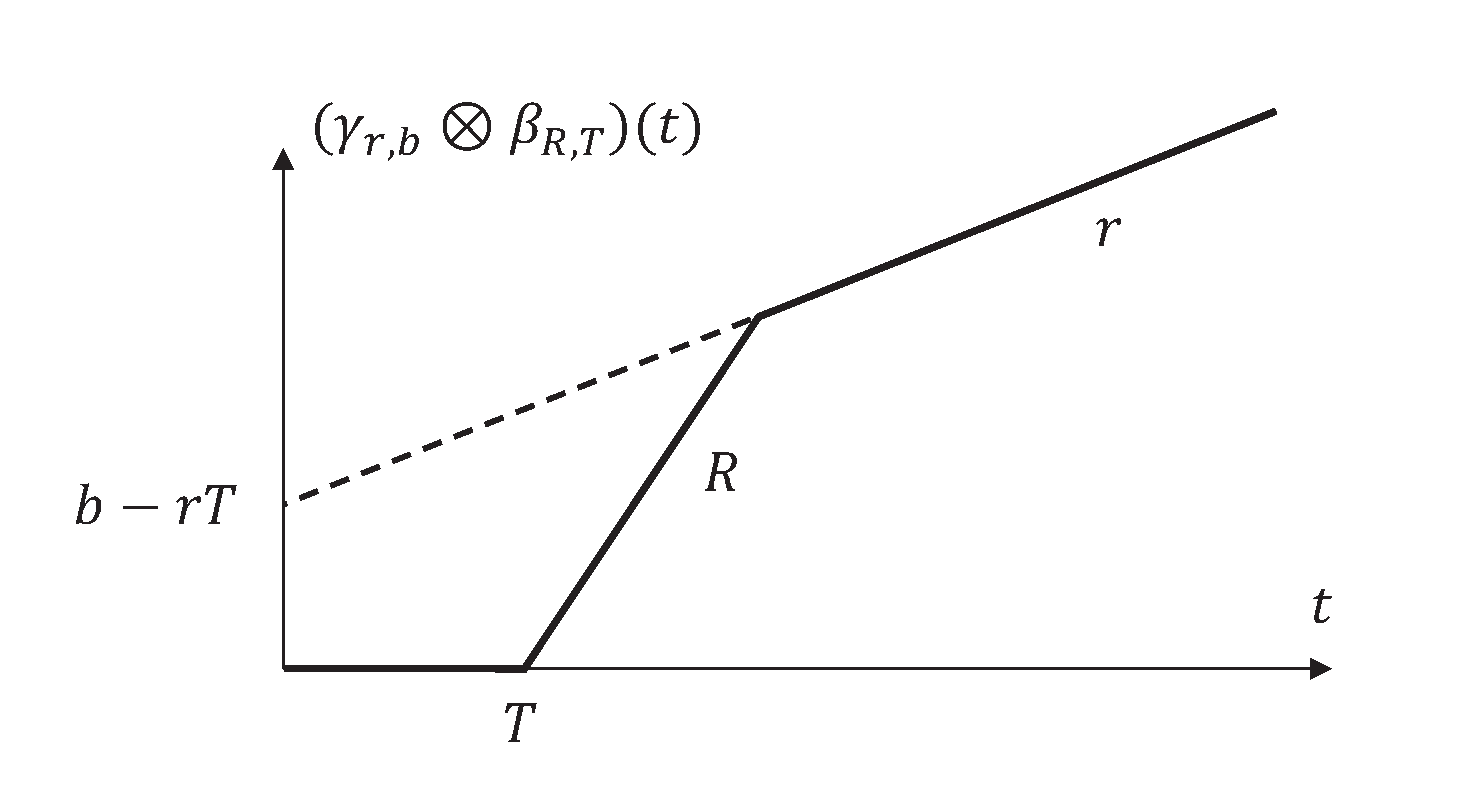
\includegraphics[width=0.7\textwidth,keepaspectratio]{ec.eps}
  \mycaption{Function $\gamma_{r,b} \otimes \beta_{R,T}$ when $0 < r < R$.}
 \mylabel{fig:exampleconvolution}
\end{figure}
Let us now derive some useful properties for the computation of min-plus convolution.
%We first begin by a set of six rules establishing a structure of commutative dioid for  $(\calF, \wedge, \otimes)$:
\begin{theorem}[General properties of $\otimes$]
\mylabel{thm:rule1-7}
Let $f, g, h \in \calF$.
\begin{itemize}
\item{\textbf{Rule 1 (Closure of $\otimes$)}
$(f \otimes g) \in \calF$.}
\item{\textbf{Rule 2 (Associativity of $\otimes$)}
$(f \otimes g) \otimes h =  f \otimes (g \otimes h)$.}
\item{ \textbf{Rule 3 (The zero element for $\wedge$ is absorbing for $\otimes$)}
The zero element for $\wedge$ belonging to $\calF$ is the function $\varepsilon$, defined as
$\varepsilon(t) = +\infty$ for all $t \geq 0$ and $\varepsilon(t) = 0$ for all $t < 0$.
One has $f \otimes \varepsilon = \varepsilon$.}
\item{ \textbf{Rule 4 (Existence of a neutral element for $\otimes$)}
The neutral element is $\delta_0$, as $f \otimes \delta_0 = f$.}
\item{ \textbf{Rule 5 (Commutativity of $\otimes$)} $f \otimes g = g \otimes f$.}
\item{ \textbf{Rule 6 (Distributivity of $\otimes$ with respect to $\wedge$)}
$(f \wedge g) \otimes h =  (f \otimes h) \wedge (g \otimes h)$. }
\item{ \textbf{Rule 7 (Addition of a constant)} For any $K \in \Reals^{+}$,
$(f + K) \otimes g =  (f \otimes g) + K$. }
\end{itemize}
\end{theorem}
The proof of these rules is easy. We prove the two first rules, the proof of the five others are
left to the reader.
%\begin{itemize}
%\item{\textbf{Rule 1 (Closure of $\otimes$)} For all $f, g \in \calF$,
%$(f \otimes g) \in \calF$.}
%\item{\textbf{Rule 2 (Associativity of $\otimes$)} For all $f, g, h \in \calF$,
%$(f \otimes g) \otimes h =  f \otimes (g \otimes h)$.}
%\item{ \textbf{Rule 3 (The zero element for $\wedge$ is absorbing for $\otimes$)}
%The zero element for $\wedge$ belonging to $\calF$ is the function $\varepsilon$, defined as
%$\varepsilon(t) = +\infty$ for all $t \geq 0$ and $\varepsilon(t) = 0$ for all $t < 0$.
%Then for all $f \in \calF$, $f \otimes \varepsilon = \varepsilon$.}
%\item{ \textbf{Rule 4 (Existence of a neutral element for $\otimes$)}
%The neutral element is $\delta_0$, as for all $f \in \calF$, $f \otimes \delta_0 = f$.}
%\item{ \textbf{Rule 5 (Commutativity of $\otimes$)} For all $f, g \in \calF$, $f \otimes g = g \otimes f$.}
%\item{ \textbf{Rule 6 (Distributivity of $\otimes$ with respect to $\wedge$)}  For all $f, g, h \in \calF$,
%$(f \wedge g) \otimes h =  (f \otimes h) \wedge (g \otimes h)$. }
%\end{itemize}
\pr (Rule 1) Since $f$ is wide-sense increasing,
$$ f(t_1-s) + g(s) \leq f(t_2-s) + g(s) $$
for all $0 \leq t_1 < t_2$ and all $s \in \Reals$. Therefore
$$ \inf_{s \in \Reals} \left\{ f(t_1-s) + g(s) \right\} \leq \inf_{s \in \Reals} \left\{ f(t_2-s) + g(s) \right\} $$
and as $f(t) = g(t) = 0$ when $t < 0$, this inequality is equivalent to
$$ \inf_{0 \leq s \leq t_1} \left\{ f(t_1-s) + g(s) \right\} \leq \inf_{0 \leq s \leq t_2} \left\{ f(t_2-s) + g(s) \right\}, $$
which shows that $(f \otimes g)(t_1) \leq (f \otimes g)(t_2)$ for all $0 \leq t_1 < t_2$.
\vspace{1ex}
\noindent
(Rule 2) One has
\begin{eqnarray*}
((f \otimes g) \otimes h)(t)
& = & \inf_{0 \leq s \leq t} \left\{ \inf_{0 \leq u \leq t-s}
        \left\{ f(t-s-u) + g(u) \right\} + h(s) \right\} \\
& = & \inf_{0 \leq s \leq t} \left\{ \inf_{s \leq u' \leq t} \left\{ f(t-u') + g(u'-s) + h(s) \right\} \right\} \\
& = & \inf_{0 \leq u' \leq t} \left\{ \inf_{0 \leq s \leq u'} \left\{ f(t-u') + g(u'-s) + h(s) \right\} \right\}  \\
& = & \inf_{0 \leq u' \leq t} \left\{  f(t-u') + \inf_{0 \leq s \leq u'} \left\{ g(u'-s) + h(s) \right\} \right\}  \\
& = & \inf_{0 \leq u' \leq t} \left\{  f(t-u') + (g \otimes h)(u') \right\}  \\
& = & (f \otimes (g \otimes h))(t).
\end{eqnarray*}
\qed

Rules 1 to 6 establish a structure of a commutative dioid for
$(\calF, \wedge, \otimes)$, whereas Rules 6 and 7 show that
$\otimes$ is a linear operation on $(\Reals^{+}, \wedge, +)$. Now
let us also complete these results by two additional rules that
are helpful in the case of concave or convex functions.
\begin{theorem}[Properties of $\otimes$ for concave/convex functions]
\mylabel{thm:rule8-9}
Let $f,g \in \calF$.
\begin{itemize}
\item{\textbf{Rule 8 (Functions passing through the origin)} If $f(0) = g(0) = 0$
then $f \otimes g \leq f \wedge g$. Moreover, if $f$ and $g$ are star-shaped,
then $f \otimes g = f \wedge g$.}
\item{\textbf{Rule 9 (Convex functions)}
If $f$ and $g$ are convex then $f \otimes g$ is convex. In particular if $f, g$
are convex and piecewise linear, $f \otimes g$ is obtained by putting end-to-end the different
linear pieces of $f$ and $g$, sorted by increasing slopes.}
\end{itemize}
\end{theorem}
Since concave functions are star-shaped, Rule~8 also implies that if $f,g$ are concave with $f(0) = g(0) =0$, then  $f \otimes g = f \wedge g$.
\pr (Rule 8) As $f(0) = g(0) = 0$,
\begin{equation}
\mylabel{eq:Rule7proof}
(f \otimes g)(t) = g(t) \wedge \inf_{0 < s < t} \left\{ f(t-s) + g(s)  \right\} \wedge f(t) \leq f(t) \wedge g(t).
\end{equation}
Suppose now that, in addition, $f$ and $g$ are star-shaped. Then for any $t > 0$ and $0 \leq s \leq t$
$f(t-s) \geq (1-s/t)f(t)$ and $g(s) \geq (s/t)g(t) $, so that
$$ f(t-s) + g(s) \geq f(t) + (s/t) (g(t) - f(t)). $$
Now, as $0 \leq s/t \leq 1$, $ f(t) + (s/t) (g(t) - f(t)) \geq f(t) \wedge g(t)$ so that
$$ f(t-s) + g(s) \geq f(t) \wedge g(t) $$
for all $0 \leq s \leq t$. Combining this inequality with (\ref{eq:Rule7proof}), we obtain the desired result.
%Suppose now that, in addition, $f$ and $g$ are concave. Then for any $u, u' \in [0,1]$
%and $x, y \geq 0$, $f(ux + (1-u)y) \geq uf(x) + (1-u)f(y)$ and $g(u'x + (1-u')y) \geq u'g(x) + (1-u')g(y)$.
%Take $x = t$, $y = 0$, $u = 1-s/t$ and $u' = s/t$, with $0 \leq s \leq t$. Then the two previous inequalities become
%$f(t-s) \geq (1-s/t)f(t)$ and $g(s) \geq (s/t)g(t) $, so that
%$$ f(t-s) + g(s) \geq f(t) + (s/t) (g(t) - f(t)). $$
%Now, as $0 \leq s/t \leq 1$, $ f(t) + (s/t) (g(t) - f(t)) \geq f(t) \wedge g(t)$ so that
%$$ f(t-s) + g(s) \geq f(t) \wedge g(t) $$
%for all $0 \leq s \leq t$. Combining this inequality with (\ref{eq:Rule7proof}), we obtain the desired result.
\vspace{1ex}
\noindent
(Rule 9) The proof uses properties of convex sets and functions listed in the previous subsection.
The epigraphs of $f$ and $g$ are the sets
\begin{eqnarray*}
\calS_1 & = & \{ (s_1,\mu_1) \in \Reals^2 \mst f(s_1) \leq \mu_1 \} \\
\calS_2 & = & \{ (s_2,\mu_2) \in \Reals^2 \mst g(s_2) \leq \mu_2 \}
\end{eqnarray*}
Since $f$ and $g$ are convex, their epigraphs are also convex, and so is their sum $\calS = \calS_1 + \calS_2$,
which can be expressed as
$$\calS = \{ (t,\mu) \in \Reals^2  | \mbox{ for some } (s,\xi) \in [0,t] \times [0,\mu], f(t-s) \leq \mu - \xi,
g(s) \leq \xi \}. $$
As $\calS$ is convex, function $h(t) = \inf \{ \mu \in \Reals \mst (t,\mu) \in \calS \}$ is also convex.
Now $h$ can be recast as
\begin{eqnarray*}
\lefteqn{ h(t) }\\ & = & \inf \{ \mu \in \Reals \; | \mbox{ for
some} (s,\xi) \in [0,t] \times [0,\mu], f(t-s) \leq \mu - \xi,
g(s) \leq \xi \} \\
    & = & \inf \{ \mu \in \Reals \; | \mbox{ for some } s \in [0,t], f(t-s) + g(s) \leq \mu \} \\
    & = & \inf \{ f(t-s) + g(s),  s \in [0,t] \} \\
    & = & (f \otimes g)(t),
\end{eqnarray*}
which proves that $(f \otimes g)$ is convex.

If $f$ and $g$ are piecewise linear, one can construct the set $\calS = \calS_1 + \calS_2$,
which is the epigraph of $f \otimes g$,
by putting end-to-end the different linear pieces of $f$ and $g$, sorted by increasing slopes
\cite{vecpri96}.

Indeed, let $h'$ denote the function that results from this
operation, and let us show that $h' = f \otimes g$. Suppose that
there are a total of $n$ linear pieces from $f$ and $g$, and label
them from $1$ to $n$ according to their increasing slopes: $0 \leq
r_1 \leq r_2 \leq \ldots \leq r_n$. Figure~\ref{fig:convexpwlsum}
shows an example for $n=5$. Let $T_i$ denote the length of the
projection of segment~$i$ onto the horizontal axis, for $1 \leq i
\leq n$. Then the length of the projection of segment~$i$ onto the
vertical axis is $r_iT_i$.
\begin{figure}[!htbp]
    \insfig{convexpwlsum}{0.85}
  \mycaption{Convex, piecewise linear functions $f$ (and its epigraph $\calS_1$ (top left)), $g$ (and its epigraph $\calS_2$
  (top right)), and $f \otimes g$ (and its epigraph $\calS = \calS_1 + \calS_2$ (bottom)).}
 \mylabel{fig:convexpwlsum}
\end{figure}
Denote by $\calS '$ the epigraph of $h'$, which is convex, and by $ \partial \calS '$ its boundary.
% (i.e., the set of points $(t,h'(t))$.)
Pick any point $(t,h'(t))$ on this boundary $\partial \calS '$. We will show that it
can always be obtained by adding a point $(t-s,f(t-s))$
of the boundary $ \partial \calS_1$ of $\calS_1$ and a point
$(s,g(s))$  of the boundary $ \partial \calS_2$ of $\calS_2$.
 Let $k$ be the linear segment index to which $(t,h'(t))$
belongs, and assume, with no loss of generality, that this segment is a piece of $f$
(that is, $k \subseteq  \partial \calS_1$).
We can express $h'(t)$ as
\begin{equation}
\mylabel{eq:h'}
 h'(t) = r_k (t - \sum_{i=1}^{k-1}T_i ) + \sum_{i=1}^{k-1}r_iT_i.
\end{equation}
Now, let $s$ be the sum of the lengths of the horizontal projections of
the segments belonging to $g$ and whose index is less than $k$, that is,
$$ s = \sum_{  i \subseteq \partial \calS_2, 1 \leq i \leq k-1} T_i. $$
Then we can compute that
\begin{eqnarray*}
 t- s & = & t - \sum_{i=1}^{k-1}T_i  + \sum_{i=1}^{k-1}T_i - \sum_{i \subseteq \partial \calS_2, 1 \leq i \leq k-1} T_i \\
    & = & t - \sum_{i=1}^{k-1}T_i  + \sum_{i \subseteq \partial \calS_1, 1 \leq i \leq k-1} T_i
\end{eqnarray*}
and that
\begin{eqnarray*}
f(t-s) & = & r_k(t - \sum_{i=1}^{k-1}T_i ) +  \sum_{ i \subseteq \partial \calS_1, 1 \leq i \leq k-1} r_i T_i \\
 g(s) & = &  \sum_{i \subseteq \partial \calS_2, 1 \leq i \leq k-1} r_iT_i.
\end{eqnarray*}
The addition of the right hand sides of these two equations is
equal to $h'(t)$, because of (\ref{eq:h'}), and therefore $f(t-s)
+ g(s) = h'(t)$. This shows that any point of $\partial \calS'$
can be broken down into the sum of a point of $\partial \calS_1$
and of a point of $\partial \calS_2$, and hence that $\partial
\calS'
=
\partial \calS_1 + \partial \calS_2$,  which in turn implies that
$\calS' = \calS_1 + \calS_2 = \calS$. Therefore $h'= f \otimes g$.
\qed

The last rule is easy to prove, and states that $\otimes$ is
isotone, namely:
\begin{theorem}[Isotonicity of $\otimes$]
\mylabel{thm:isotonicityofconvolution}
Let $f, g, f', g' \in \calF$.
\begin{itemize}
\item{\textbf{Rule 10 (Isotonicity)} If $f \leq g$ and $f' \leq g'$ then $f \otimes f' \leq  g \otimes g'$.}
\end{itemize}
\end{theorem}
We will use the following theorem:
\begin{theorem}
\mylabel{theo-minplust0} For $f$ and $g$ in $\calF$, if in
addition $g$ is continuous, then for any $t$ there is some $t_0$
such that
\begin{equation}\mylabel{eq-sercur-d2}
 (f \mpc g)(t)= f_l(t_{0}) + g(t-t_{0})
\end{equation}
where $f_l(t_0)= \sup_{\{s < t_0\}} f(s)$ is the limit from the left
of $f$ at $t_0$. If $f$ is left-continuous, then
$f_l(t_0)=f(t_0)$.
\end{theorem}
\pr
Fix $t$. There is a sequence of times $0 \leq s_n \leq t$ such
that
\begin{equation}\mylabel{eq-sercurconti}
  \inf_{t_0
\leq t} \left(f(t_{0})  + g(t-t_{0})\right) = \lim_{n \rightarrow
\infty} \left(f(s_{n})  + g(t-s_{n})\right)
\end{equation}
Since $0\leq s_n \leq t$, we can extract a sub-sequence that
converges towards some value $t_0$. We take a notation shortcut
and write $\lim_{n \rightarrow \infty} s_n=t_0$. If $f$ is
continuous, the right hand-side in \ref{eq-sercurconti} is equal
to $f_l(t_{0}) + g(t-t_{0})$ which shows the proposition.
Otherwise $f$ has a discontinuity at $t_0$. Define
$\delta=f(t_0)-f_l(t_0)$.  We show that we can again extract a
subsequence such that $s_n < t_0$. Indeed, if this would not be
true, we would have $s_n \geq t_0$ for all  but a finite number of
indices $n$. Thus for $n$ large enough we would have
 $$f(s_n)  \geq f_l(t_0)+ \delta $$
 and by
continuity of $g$:
$$
 g(t-s_n) \geq g(t-t_0) -\frac{\delta}{2}
 $$ thus
 $$
 f(s_n)+ g(t-s_{n}) \geq f_l(t_0)+ g(t-t_0) +\frac{\delta}{2}
 $$
 Now $$ f_l(t_0)+ g(t-t_0) \geq \inf_{s
\leq t} \left(f(s)  + g(t-s)\right)$$ thus
$$
 f(s_n)+ g(t-s_{n}) \geq \inf_{s
\leq t} \left(f(s)  + g(t-s)\right) +\frac{\delta}{2}
$$
 which contradicts \ref{eq-sercurconti}.
 Thus we can assume that $s_n \leq t_0$ for $n$ large enough and
 thus $\lim_{n
\rightarrow \infty} f(s_{n})= f_l(t_0)$. \qed

Finally, let us mention that it will sometimes be useful to break
down a somewhat complex function into the convolution of a number
of simpler functions. For example, observe that the rate-latency
function $\beta_{R,T}$ can be expressed as
\begin{equation}
\mylabel{eq:ratelatencydecomposition}
 \beta_{R,T} = \delta_{T} \otimes \lambda_{R}.
\end{equation}

%Suppose that $f$ and $g$ are convex, and let $F(t,s) = f(t-s) + g(s)$.
%Let $u \in [0,1]$ and $x, y \geq 0$. Then
%\begin{eqnarray*}
%F((1-u)x + uy,(1-u)x' + uy') & = & f((1-u)(x-x') + u(y-y')) + g((1-u)x' + uy') \\
%          & \leq &  ((1-u)f(x-x') + uf(y-y')) + (1-u)g(x') + ug(y') \\
%       & = &  (1-u)(f(x-x') + g(x')) + u(f(y-y') + g(y')) = (1-u)F(x,x') + uF(y,y')
%\end{enqarray*}
%which shows that $F$ is a convex function from $\Reals^2$ to $Reals^{+}$.
\subsection{Sub-additive Functions}
\mylabel{sec:sub-additivefunctions}
\index{sub-additive fucntion}
Another class of functions will be important in network calculus are sub-additive functions, which
are defined as follows.
\begin{definition}[Sub-additive function]
\mylabel{def:sub-additivefunction}
Let $f$ be a function or a sequence of $\calF$. Then $f$ is sub-additive if and only if $f(t+s) \leq f(t) + f(s)$
for all $s,t \geq 0$.
\end{definition}
Note that this definition is equivalent to imposing that $f \leq f \otimes f$. If $f(0)=0$, it is equivalent
to imposing that $f \otimes f = f$.

We will see in the following theorem that concave functions passing through the origin are sub-additive.
So the piecewise linear function $f_1$ given by (\ref{eq:pwlconcave}), being concave and passing through
the origin, is sub-additive.

The set of sub-additive functions is however larger than that of concave functions:
 the piecewise linear function $f_2$ given by (\ref{eq:pwlsubadditive}) is not concave, yet one check
that it verifies Definition~\ref{def:sub-additivefunction} and hence is sub-additive.

Contrary to concave and convex functions, it is not always
obvious, from a quick visual inspection of the graph of a
function, to establish whether it is sub-additive or not. Consider
the two functions $ \beta_{R,T} + K'$ and $\beta_{R,T} + K''$,
represented respectively on the left and right of
Figure~\ref{fig:betaplusRT}. Although they differ only by the
constants $K'$ and $K''$, which are chosen so that $0 < K'' < RT <
K' < +\infty$, we will see $\beta_{R,T} + K'$ is sub-additive but
not $\beta_{R,T} + K''$.
\begin{figure}[!htbp]
\insfig{betaplusRT}{0.8}
\mycaption{Functions $\beta_{R,T} + K'$ (left) and $\beta_{R,T} + K''$ (right). The only difference between them
is the value of the constant: $ K'' < RT < K' $.}
\mylabel{fig:betaplusRT}
\end{figure}
Consider first  $\beta_{R,T} + K'$.
If $s +t \leq T$, then $s,t \leq T$ and
$$\beta_{R,T}(s+t) + K' = K' < 2K' = (\beta_{R,T}(s) + K') + (\beta_{R,T}(t) + K'). $$
On the other hand, if $s +t > T$, then,  since $K' > RT$,
\begin{eqnarray*}
\beta_{R,T}(t+s) + K' & = & R(t+s-T) + K' \\
              & < & R(s+t-T) + K' + (K'-RT)  \\
              &  = & (R(t-T) + K') + (R(s-T) + K') \\
              & \leq & (\beta_{R,T}(t) + K') + (\beta_{R,T}(s) + K'),
\end{eqnarray*}
which proves that $\beta_{R,T} + K'$ is sub-additive.
Consider next $\beta_{R,T} + K''$. Pick $s = T$ and $t > T$. Then, since $K'' < RT$,
%\begin{eqnarray*}
%\beta_{R,T}(t+s) + K'' & = & \beta_{R,T}(t+T) + K'' = Rt + K'' =
%R(t-T) + RT + K'' \\
%               & > & R(t-T) + K'' + K''
%                = (\beta_{R,T}(t) + K'') + (\beta_{R,T}(s) + K''),
%\end{eqnarray*}
\begin{eqnarray*}
\lefteqn{\beta_{R,T}(t+s) + K''  =}\\
 & & \beta_{R,T}(t+T) + K'' = Rt + K'' = R(t-T) + RT + K'' \\
 &  & >  R(t-T) + K'' + K''
                = (\beta_{R,T}(t) + K'') + (\beta_{R,T}(s) + K''),
\end{eqnarray*}
which proves that $\beta_{R,T} + K''$ is not sub-additive.

Let us list now some properties of sub-additive functions.
\begin{theorem}[Properties of sub-additive functions]
\mylabel{thm:propertiessub-additivefunction}
Let $f,g \in \calF$.
\begin{itemize}
\item{\textbf{(Star-shaped functions passing through the origin)} If $f$ is star-shaped with $f(0) = 0$,
then $f$ is sub-additive.}
\item{\textbf{(Sum of sub-additive functions)} If $f$ and $g$ are sub-additive, so is $(f + g)$.}
\item{ \textbf{(Min-plus convolution of sub-additive functions)} If  $f$ and $g$ are sub-additive,
so is $(f \otimes g)$.}
%\item{\textbf{(Definition of sub-additivity using min-plus convolution)} Let $f$ be such that $f(0) = 0$.
%Then $f$ is  sub-additive if and only if $f \otimes f = f$}
\end{itemize}
\end{theorem}
The first property also implies that concave functions passing through the origin are sub-additive. The proof of the second property is simple and left to the reader, we prove the two others.
\pr (Star-shaped functions passing through the origin)
Let $s,t \geq 0$ be given. If $s$ or $t=0$, one clearly
 has that $f(s+t) = f(s) + f(t)$.
Assume next that $s, t > 0$. As $f$ is star-shaped,
\begin{eqnarray*}
f(s) &  \geq &  \frac{s}{s+t} f(s+t) \\
f(t) &  \geq &  \frac{t}{s+t} f(s+t)
\end{eqnarray*}
which sum up to give $ f(s) + f(t) \geq f(s+t) $.
\vspace{1ex}
\noindent
(Min-plus convolution of sub-additive functions)
Let $s,t \geq 0$ be given. Then
\begin{eqnarray*}
\lefteqn{(f \otimes g)(s) + (f \otimes g)(t)} \\
 & = & \inf_{0 \leq u
\leq s} \left\{ f(s -u) + g(u) \right\} + \inf_{0 \leq v \leq t}
\left\{ f(t -v) + g(v) \right\} \\
        & = & \inf_{0 \leq u \leq s} \inf_{0 \leq v \leq t} \left\{ f(s -u) + f(t-v) + g(u) + g(v) \right\} \\
        & \geq & \inf_{0 \leq u \leq s} \inf_{0 \leq v \leq t} \left\{ f(s+t -(u+v)) + g(u + v) \right\} \\
        & = & \inf_{0 \leq u+v \leq s+t} \left\{ f(s+t -(u+v)) + g(u + v) \right\} \\
        & = & (f \otimes g)(t + s).
\end{eqnarray*}
%\begin{eqnarray*}
%(f \otimes g)(s) + (f \otimes g)(t) & = & \inf_{0 \leq u \leq s} \left\{ f(s -u) + g(u) \right\} + \inf_{0 \leq v \leq t} \left\{ f(t -v) + g(v) \right\} \\
%        & = & \inf_{0 \leq u \leq s} \inf_{0 \leq v \leq t} \left\{ f(s -u) + f(t-v) + g(u) + g(v) \right\} \\
%        & \geq & \inf_{0 \leq u \leq s} \inf_{0 \leq v \leq t} \left\{ f(s+t -(u+v)) + g(u + v) \right\} \\
%        & = & \inf_{0 \leq u+v \leq s+t} \left\{ f(s+t -(u+v)) + g(u + v) \right\} \\
%        & = & (f \otimes g)(t + s).
%\end{eqnarray*}
%
%\vspace{1ex}
%\noindent
%(Definition of sub-additivity using min-plus convolution)
%Suppose first that $f$ is sub-additive. Then for all $s \in [0,t]$, $f(t) \leq f(t-s) + f(s)$,
%which implies that $f(t) \leq \inf_{0 \leq s \leq t} \{ f(t-s) + f(s) \} = (f \otimes f)(t) $.
%On the other hand, $(f \otimes f)(t) =  f(t) \wedge \inf_{0 < s < t} \{ f(t-s) + f(s) \} \leq f(t)$,
%so that  $(f \otimes f)(t) =  f(t)$.
%
%Suppose next that $(f \otimes f)(t) =  f(t)$. Then for all $t \geq 0$ and all $s \in [0,t]$,
%$f(t) \leq f(t-s) + f(s)$, which shows that $f$ is sub-additive.
%
\qed

The minimum of any number of star-shaped (resp. concave) functions
is still a star-shaped (resp. concave) function. If one of them
passes through the origin, it is therefore a sub-additive
function: for example, as already mentioned earlier, the concave
piecewise linear function $f_1$ given by (\ref{eq:pwlconcave}) is
sub-additive. On the other hand the minimum of two sub-additive
functions is not, in general, sub-additive. Take for example the
minimum between a rate latency function $\beta_{R',T}$ and
function $f_2$ given by (\ref{eq:pwlsubadditive}), when $R' =
2R/3$. with $R, T$ as defined in (\ref{eq:pwlsubadditive}).
 Both functions are sub-additive, but one can check that $\beta_{R',T} \wedge f_2$ is not.

The first property of the previous theorem tells us that all
star-shaped functions are sub-additive. One can check for example
that $\beta_{R,T} + K'$ is a star-shaped function (which is not
concave), but not $\beta_{R,T} + K''$. One can also wonder if,
conversely, all sub-additive functions are star-shaped. The answer
is no: take again
 function $f_2$ given by (\ref{eq:pwlsubadditive}), which is sub-additive. It is not star-shaped, because
$f(2T)/2T = R/2 < 2R/3 = f(3T)/3T$.
\subsection{Sub-additive Closure}
\mylabel{sec:sub-additiveclosure}
\index{1sub-additiveclosure@$\overline{f}$ (sub-additive closure of $f$)}
\index{sub-additive closure}

Given a function $f \in \cal F$, if $f(0) = 0$, then $f \geq f
\otimes f \geq 0$. By repeating this operation, we will get a
sequence of functions that are each time smaller (in the wide sense) and converges to
some limiting function that, as we will see, is the largest
sub-additive function smaller than $f$ (in the wide sense) and zero in $t=0$, and is
called sub-additive closure of~$f$. The formal definition is as
follows.
\begin{definition}[Sub-additive closure]
\mylabel{def:sub-additiveclosure}
Let $f$ be a function or a sequence of $\calF$. Denote $f^{(n)}$ the function obtained
by repeating $(n-1)$ convolutions of $f$ with itself. By convention, $f^{(0)} = \delta_0$,
so that $f^{(1)} = f$, $f^{(2)} = f \otimes f$, etc.
Then the sub-additive closure of $f$,  denoted by $\overline{f}$, is defined by
\begin{equation}
\mylabel{eq:sub-additiveclosure}
\overline{f} = \delta_0 \wedge f \wedge (f \otimes f) \wedge (f \otimes f \otimes f) \wedge \ldots = \inf_{n \geq 0} \left\{ f^{(n)} \right\}.
\end{equation}
\end{definition}
\noindent
{\bf Example.} Let us compute the sub-additive closure of the two functions $\beta_{R,T} + K'$ and $\beta_{R,T} + K''$, represented respectively on the left and right
of Figure~\ref{fig:betaplusRT}. Note first that Rule~7 of Theorem~\ref{thm:rule1-7} and
Rule~9 of Theorem~\ref{thm:rule8-9}  yield that for any $K > 0$,
$$ (\beta_{R,T} + K) \otimes (\beta_{R,T} + K) = ( \beta_{R,T} \otimes \beta_{R,T}) + 2K = \beta_{R,2T} + 2K.$$
Repeating this convolution $n$ times yields that for all integers $n \geq 1$
$$ (\beta_{R,T} + K)^{(n)} = \beta_{R,nT} + nK . $$
Now, if $K = K' > RT$ and $t \leq nT$,
\begin{eqnarray*}
 \beta_{R,nT} + nK' & = & nK' > (n-1)RT + K' = R(nT - T) + K' \\
        & \geq & R[t-T]^{+} + K' = \beta_{R,T} + K',
 \end{eqnarray*}
whereas if $t > nT$
\begin{eqnarray*}
 \beta_{R,nT} + nK' &  =  & R(t-nT) + nK' = R(t-T) + (n-1)(K'-RT) + K' \\
        & > &  R(t-T) + K' =  \beta_{R,T} + K'
 \end{eqnarray*}
%
%$$ \beta_{R,nT}) + nK' = \left\{ \begin{array}{lll} %nK' > K' = R[t-T]^{+} + K' & \mbox{ if } t \leq T \\
%           nK' > (n-1)RT + K' \geq R[t-T]^{+} + K'  & \mbox{ if } & t \leq nT \\
%           R(t-nT) + nK' = R(t-T) + (n-1)(K'-RT) + K' > R[t-T]^{+} + K'  & \mbox{ if } & t > nT \end{array} \right. $$
%
so that $ (\beta_{R,T} + K')^{(n)} \geq \beta_{R,T} + K'$ for all $n \geq 1$. Therefore (\ref{eq:sub-additiveclosure})
becomes
$$ \overline{\beta_{R,T} + K' } = \delta_0 \wedge \inf_{n \geq 1} \left\{ (\beta_{R,T} + K')^{(n)} \right\} =
\delta_0 \wedge (\beta_{R,T} + K'), $$
and is shown on the left of Figure~\ref{fig:betaplusRTclosure}.
On the other hand, if $K = K'' < RT$, the infimum in the previous equation is not reached in $n = 1$ for every $t > 0$,
so that the sub-additive closure is now expressed by
$$ \overline{\beta_{R,T} + K'' } = \delta_0 \wedge \inf_{n \geq 1} \left\{ (\beta_{R,T} + K'')^{(n)} \right\} =
\delta_0 \wedge \inf_{n \geq 1} \left\{ (\beta_{R,nT} + nK'') \right\}, $$
and is shown on the right of Figure~\ref{fig:betaplusRTclosure}.
\begin{figure}[!htbp]
   \insfig{betaplusRTclosure}{0.8}
  \mycaption{The sub-additive closure of functions $\beta_{R,T} + K'$ (left) and $\beta_{R,T} + K''$ (right), when $K'' < RT < K'$.}
 \mylabel{fig:betaplusRTclosure}
 \end{figure}

Among all the sub-additive functions that are smaller (in the wide sense) than $f$ and
that are zero in $t=0$, there is one that is an upper bound for
all others; it is equal to $\overline{f}$, as established by the
following theorem.
\begin{theorem}[Sub-additive closure]
\mylabel{thm:sub-additiveclosure}
Let $f$ be a function or a sequence of $\calF$, and let $\overline{f}$ be its sub-additive closure.
Then
\noindent
(i)  $\overline{f} \leq f$, $\overline{f} \in \calF$ and $\overline{f}$ is sub-additive.
\noindent
(ii) if function $g \in \calF$ is sub-additive, with $g(0) = 0$ and $g \leq f$, then $g \leq \overline{f}$.
\end{theorem}
\pr (i) It is obvious from Definition~\ref{def:sub-additiveclosure}, that $\overline{f} \leq f$. By repeating
$(n-1)$ times Rule~1 of Theorem~\ref{thm:rule1-7}, one has that $f^{(n)} \in \calF$ for all $n \geq 1$.
As $f^{(0)}  = \delta_0 \in \calF$ too, $\overline{f} = \inf_{n \geq 0} \{ f^{(n)} \} \in \calF$.
Let us show next that $\overline{f}$ is sub-additive. For any integers $n,m \geq 0$, and for any $s,t \geq 0$,
\begin{eqnarray*}
f^{(n+m)}(t+s) & = & (f^{(n)} \otimes f^{(m)})(t+s) = \inf_{0 \leq u \leq t+s} \{ f^{(n)}(t+s-u) + f^{(m)}(u) \}\\
        & \leq & f^{(n)}(t) + f^{(m)}(s)
\end{eqnarray*}
so that
\begin{eqnarray*}
\overline{f}(t+s) & = & \inf_{n+m\geq 0} \{ f^{(n+m)}(t+s) \} = \inf_{n,m\geq 0} \{ f^{(n+m)}(t+s) \}  \\
            & \leq & \inf_{n,m\geq 0} \{ f^{(n)}(t) + f^{(m)}(s) \} \\
        & = & \inf_{n\geq 0} \{ f^{(n)}(t) \} +
            \inf_{m \geq 0} \{f^{(m)}(s) \} = \overline{f}(t) + \overline{f}(s)
\end{eqnarray*}
which shows that $\overline{f}$ is sub-additive.
(ii) Next, suppose that $g \in \calF$ is sub-additive, $g(0) = 0$ and $g \leq f$.
Suppose that for some $n \geq 1$,  $f^{(n)} \geq g$.
Clearly, this holds for $n = 0$ (because $g(0) = 0$ implies that $g \leq \delta_0 = f^{(0)}$) and for $n =1$.
Now, this assumption and the sub-additivity of $g$ yield that for any $0 \leq s \leq t$,
$f^{(n)}(t-s) + f(s) \geq g(t-s) + g(s) \geq g(t)$ and hence that $f^{(n+1)}(t) \geq g(t)$.
By recursion on $n$, $f^{(n)} \geq g$  for all $n \geq 0$, and therefore $\overline{f} = \inf_{n \geq 0} \{ f^{(n)} \}
 \geq g$.
\qed
\begin{corollary}[Sub-additive closure of a sub-additive function]
\mylabel{cor:sub-additiveclosure}
Let $f \in \calF$. Then the three following statements are equivalent:
(i) $f(0)=0$ and $f$ is sub-additive
(ii) $f \otimes f = f$
(iii) $\overline{f} = f$.
\end{corollary}
\pr (i) $\Rightarrow $ (ii) follows immediately from from Definition~\ref{def:sub-additivefunction}.
(ii) $\Rightarrow $ (iii): first note that $f \otimes f = f$ implies that $f^{(n)} = f$ for all $n \geq 1$.
Second, note that $(f \otimes f)(0) = f(0) + f(0) $, which implies that $f(0) = 0$. Therefore
$\overline{f} = \inf_{n \geq 0} \{ f^{(n)} \} = \delta_0 \wedge f = f$.
(iii) $\Rightarrow $ (i) follows from Theorem~\ref{thm:sub-additiveclosure}.
\qed
%The usefulness of the sub-additive closure lies from the fact that if a function $f$ is constrained by a function
%then it is also constrained by the sub-additive closure
%of $g$, as proven by from the following theorem. Such constrains will occur frequently for
%characterizing the burstiness of a traffic flow in the next chapters.
%\begin{theorem}[Function with a constraint on sliding windows]
%\mylabel{thm:sub-additiveclosureconstraint}
%Let $f,g \in \cal F$. Then
%$$ f \leq f \otimes g \;\;\;\; \mbox{ if and only if } \;\;\;\; f \leq f \otimes \overline{g}. $$
%\end{theorem}
%
%
%\pr The `if' part is obvious from the definition of sub-additive closure (\ref{eq:sub-additiveclosure})
%and the property of isotonicity of
%$\otimes$ (Rule 10), so we need only to prove the `only if' part of the theorem.
%As we assume that $f(t) \leq (f \otimes g)(t)$
%for all $t \geq 0$, it implies that for any $ v \in [0,t]$
%$$ f(t) - f(v) \leq (f \otimes g)(t) - f(v) \leq (f(v) + g(t-v)) - f(v) = g(t-v) $$
%and hence that for all $0 \leq s \leq u \leq t$
%$$f(t) - f(s) = (f(t) - f(u)) + (f(u) - f(s)) \leq g(t-u) + g(u-s). $$
%Since the latter is true for any $u \in [s,t]$, it is equivalent to imposing that
%$$ f(t) - f(s) \leq  \inf_{s \leq u \leq t} \left\{ g(t-u) + g(u-s) \right\} =
%       % \inf_{0 \leq u' \leq t-s} \left\{ g(t-s-u') + g(u') \right\}
%       = (g \otimes g)(t-s). $$
%Now suppose that we have proven that for some $n \geq 1$, $f(t) - f(s) \leq g^{(n)}(t-s)$.
%Then
%$$ f(t) - f(s) = (f(t) - f(u)) + (f(u) - f(s)) \leq g(t-u) + g^{(n)}(u-s) $$
%and since the latter is true for any $u \in [s,t]$, it is equivalent to imposing that
%$$ f(t) - f(s) \leq  \inf_{s \leq u \leq t} \left\{ g(t-u) + g^{(n)}(u-s) \right\} =
%       (g \otimes g^{(n)})(t-s) = g^{(n+1)}(t-s) . $$
%Noting that for $n=0$, $f(t) - f(s) \leq g^{(0)}(t-s) = \delta_0(t-s)$, we have therefore proven by recurrence that
%$ f(t) - f(s) \leq g^{(n)}(t-s)$ for all $n \geq 0$ and hence that $ f(t) - f(s) \leq \overline{g} (t-s) $. \qed

The following theorem establishes some additional useful properties of the sub-additive closure of a function.
\begin{theorem}[Other properties of sub-additive closure]
\mylabel{thm:propertiessub-additiveclosure}
Let $f,g \in \calF$
\begin{itemize}
\item{\textbf{(Isotonicity)} If $f \leq g$ then $\overline{f} \leq \overline{g}$.}
\item{\textbf{(Sub-additive closure of a minimum)} $\overline{f \wedge g} = \overline{f} \otimes \overline{g}$.}
\item{\textbf{(Sub-additive closure of a convolution)} $\overline{f \otimes g} \geq \overline{f} \otimes \overline{g}$.
If $f(0) = g(0) =0$ then  $\overline{f \otimes g} = \overline{f} \otimes \overline{g}$.}
\end{itemize}
\end{theorem}
\pr (Isotonocity) Suppose that we have shown that  for some $n \geq 1$,  $f^{(n)} \leq g^{(n)}$
(Clearly, this holds for $n = 0$ and for $n =1$). Then applying Theorem~\ref{thm:isotonicityofconvolution}
we get
$$ f^{(n+1)} = f^{(n)} \otimes f \leq  g^{(n)} \otimes g = g^{(n+1)}, $$
which implies by recursion on $n$ that $\overline{f} \leq \overline{g}$.
\vspace{1ex}
\noindent
(Sub-additive closure of a minimum) One easily shows, using Theorem~\ref{thm:rule1-7},
that
$$(f \wedge g)^{(2)} = (f \otimes f) \wedge (f \otimes g) \wedge (g \otimes g).$$
Suppose that we have shown that for some $n \geq 0$, the expansion
of $ (f \wedge g)^{(n)}$ is
\begin{eqnarray*}
 \lefteqn{(f \wedge g)^{(n)} = } \\
 & & f^{(n)} \wedge (f^{(n-1)} \otimes g) \wedge (f^{(n-2)} \otimes
g^{(2)}) \wedge \ldots \wedge g^{(n)} =
\\ & & \inf_{0 \leq k \leq n} \left\{ f^{(n-k)} \otimes  g^{(k)}
\right\}.
    \end{eqnarray*}
Then
\begin{eqnarray*}
(f \wedge g)^{(n+1)}  & = & (f \wedge g) \otimes (f \wedge g)^{(n)} = \left\{ f \otimes (f \wedge g)^{(n)} \right\} \wedge
                \left\{ g \otimes (f \wedge g)^{(n)} \right\} \\
            & = & \inf_{0 \leq k \leq n} \left\{ f^{(n+1-k)} \otimes  g^{(k)} \right\} \wedge
            \inf_{0 \leq k \leq n} \left\{ f^{(n-k)} \otimes  g^{(k+1)} \right\} \\
            & = & \inf_{0 \leq k \leq n} \left\{ f^{(n+1-k)} \otimes  g^{(k)} \right\} \wedge
            \inf_{1 \leq k' \leq n+1} \left\{ f^{(n+1-k')} \otimes  g^{(k')} \right\} \\
            & = &   \inf_{0 \leq k \leq n+1} \left\{ f^{(n+1-k)} \otimes  g^{(k)} \right\}
\end{eqnarray*}
which establishes the recursion for all $n \geq 0$. Therefore
\begin{eqnarray*}
\overline{ f \wedge g} & = & \inf_{n \geq 0} \inf_{0 \leq k \leq n} \left\{ f^{(n-k)} \otimes  g^{(k)} \right\}
             =  \inf_{k \geq 0} \inf_{n \geq k} \left\{ f^{(n-k)} \otimes  g^{(k)} \right\} \\
            & = &  \inf_{k \geq 0} \inf_{l \geq 0} \left\{ f^{(l)} \otimes  g^{(k)} \right\}
             =  \inf_{k \geq 0} \left\{ \inf_{l \geq 0} \{ f^{(l)} \} \otimes  g^{(k)} \right\} \\
            & = & \inf_{k \geq 0} \left\{ \overline{f} \otimes  g^{(k)} \right\}
             =  \overline{f} \otimes \inf_{k \geq 0} \{ g^{(k)} \} =
                 \overline{f} \otimes  \overline{g}.
\end{eqnarray*}

%First, one easily shows, using the same recurrence as above,
%that for all $n \geq 0$,
%$$ (f \wedge \delta_0)^{(n)} = \delta_0 \wedge f \wedge f^{(2)} \wedge \ldots f^{(n)} =
%\min_{0 \leq i \leq n} \left\{ f^{(i)} \right\} $$
%so that
%\begin{equation}
%\mylabel{eq:resulttempof0}
%\overline{ f \wedge \delta_0 } = \overline{ f }.
%\end{equation}
%
%Now, as $(f \wedge \delta_0)(0) = (g \wedge \delta_0)(0) = 0$,  Rule 8 in Theorem~\ref{thm:rule8-9} yields
%that $(f \wedge \delta_0) \wedge (g \wedge \delta_0) = (f \wedge \delta_0) \otimes (g \wedge \delta_0)$.
%As we have shown above, $\overline{(f \wedge \delta_0) \otimes (g \wedge \delta_0)} = \overline{(f \wedge \delta_0)}
%\otimes \overline{(g \wedge \delta_0)}$, so that combining this results with (\ref{eq:resulttempof0}), we get
%\begin{eqnarray*}
%\overline{ f \wedge g} & = & \overline{ f \wedge g \wedge \delta_0} =
%           \overline{ (f \wedge \delta_0) \wedge (g \wedge \delta_0)}
%            =  \overline{ (f \wedge \delta_0) \otimes (g \wedge \delta_0)} \\
%           & = &  \overline{(f \wedge \delta_0)} \otimes \overline{(g \wedge \delta_0)}
%            = \overline{f} \otimes \overline{g}.
%\end{eqnarray*}
\vspace{1ex}
\noindent
(Sub-additive closure of a convolution)
Using the same recurrence argument as above, one easily shows that $(f \otimes g)^{(n)} = f^{(n)} \otimes g^{(n)}$,
and hence that
%
%Suppose that we have shown that  for some $n \geq 1$,  $(f \otimes g)^{(n)} = f^{(n)} \otimes g^{(n)}$
%(Clearly, this holds for $n = 0$ and for $n =1$). Then as $\otimes$
%is commutative and associative,
%\begin{eqnarray*}
%(f \otimes g)^{(n+1)} & = & (f \otimes g)^{(n)} \otimes (f \otimes g) \\
%           & = & (f^{(n)} \otimes g^{(n)}) \otimes (f \otimes g) \\
%           & = & (f^{(n)} \otimes f) \otimes (g^{(n)} \otimes g) \\
%           & = & f^{(n+1)} \otimes g^{(n+1)}
%\end{eqnarray*}
%which establishes the recursion. Therefore
%
\begin{eqnarray}
\overline{f \otimes g} & = & \inf_{n \geq 0} \left\{ (f \otimes g)^{(n)} \right\} =
                \inf_{n \geq 0} \left\{ f^{(n)} \otimes g^{(n)} \right\} \nonumber \\
            & \geq &  \inf_{n,m \geq 0} \left\{ f^{(n)} \otimes g^{(m)} \right\} \nonumber \\
            & = &   \left( \inf_{n \geq 0} \left\{ f^{(n)} \right\} \right) \otimes
              \left( \inf_{m \geq 0} \left\{ g^{(m)} \right\} \right) = \overline{f} \otimes \overline{g}.
        \mylabel{eq:resulttempclosure}
\end{eqnarray}
If $f(0) = g(0) =0$, %then $f^{(n)}(0) = g^{(n)}(0) = 0$ for all $n \geq 0$, and
Rule~8 in Theorem~\ref{thm:rule8-9} yields that $f \otimes g \leq f \wedge g$, and therefore
 that $ \overline{f \otimes g} \leq \overline{ f \wedge g } $. Now we have just shown above that
 $\overline{f \wedge g} = \overline{f} \otimes \overline{g}$, so that
 $$ \overline{f \otimes g} \leq \overline{f} \otimes \overline{g}. $$
%
%
%that $ f^{(n)} \otimes g^{(n)} \leq  f^{(n)} \wedge g^{(n)}$. In this case,
%\begin{eqnarray*}
%\overline{f \otimes g} & = & \inf_{n \geq 0} \left\{ (f \otimes g)^{(n)} \right\} =
%               \inf_{n \geq 0} \left\{ f^{(n)} \otimes g^{(n)} \right\} \\
%            & \leq &    \inf_{n \geq 0} \left\{ f^{(n)} \wedge g^{(n)} \right\} \\
%           & = &   \left( \inf_{n \geq 0} \left\{ f^{(n)} \right\} \right) \otimes
%             \left( \inf_{m \geq 0} \left\{ g^{(m)} \right\} \right) = \overline{f} \otimes \overline{g}.
%\end{eqnarray*}
 Combining this result with (\ref{eq:resulttempclosure}), we get
 $\overline{f \otimes g} = \overline{f} \otimes \overline{g}$.
\qed

Let us conclude this section with an example illustrating the
effect that a difference in taking $t$ continuous or discrete may
have. This example is the computation of the sub-additive closure
of
$$ f(t) = \left\{ \begin{array}{ccc} t^2 & \mif & t > 0 \\
                    0 & \mif & t \leq 0 \end{array} \right.  $$
Suppose first that $t \in \Reals$. Then we compute that
$$ (f \otimes f)(t) = \inf_{0 \leq s \leq t} \left\{ (t-s)^2 + s^2 \right\} = (t/2)^2 + (t/2)^2 = t^2/2 $$
as the infimum is reached in $s = t/2$. By repeating this operation $n$ times, we obtain
\begin{eqnarray*} \lefteqn{f^{(n)}(t)  = \inf_{0 \leq s \leq t} \left\{ (t-s)^2 +
(f^{(n-1)})^2(s) \right\} = } \\
 & &  \inf_{0 \leq s \leq t} \left\{
 (t-s)^2 + s^2/(n-1) \right\}  = t^2/n
 \end{eqnarray*}
as the infimum is reached in $s = t(1-1/n)$. Therefore
$$ \overline{f} (t) = \inf_{n \geq 0} \{ t^2/n \} = \lim_{n \rightarrow \infty} t^2/n = 0.$$
Consequently, if $t \in \Reals$, the sub-additive closure of function~$f$ is
$$  \overline{f} = 0, $$
as shown on the left of Figure~\ref{fig:t2closure}.
\begin{figure}[!htbp]
   \insfig{t2closure}{0.8}
  \mycaption{The sub-additive closure of $f(t) = t\lambda_1(t)$, when $t \in \Reals$ (left)
   and when $t \in \Ints$ (right).}
 \mylabel{fig:t2closure}
 \end{figure}

Now, if  $t \in \Ints$, the sequence $f(t)$ is convex and piecewise linear, as we can always connect
 the different successive points $(t, t^2)$ for all $t = 0, 1, 2, 3, \ldots $: the resulting graph
 appears as a succession of segments of slopes equal to $(2t + 1)$ (the first segment in particular has slope 1),
 and of projections on the horizontal axis having a length equal to 1, as shown on the right of
  Figure~\ref{fig:t2closure}.
 Therefore we can apply Rule~9 of Theorem~\ref{thm:rule8-9}, which yields that $f \otimes f$ is
 obtained by doubling the length of the different linear segments of $f$,
 and putting them end-to-end by increasing slopes. The analytical expression of the resulting sequence is
 $$ (f \otimes f)(t) = \min_{0 \leq s \leq t} \left\{ (t-s)^2 + s^2 \right\} = \lceil t^2/2 \rceil . $$
Sequence $f^{(2)} = f \otimes f $ is again convex and piecewise linear. Note the first segment has slope $1$,
but has now a double length. If we repeat $n$ times this convolution, it will result in a convex,
piecewise linear sequence $ f^{(n)}(t) $ whose first segment has slope~1 and horizontal length $n$:
$$ f^{(n)}(t) = t  \;\;\;\;\mif 0 \leq t \leq n, $$
as shown on the right of  Figure~\ref{fig:t2closure}.
Consequently, the sub-additive closure of sequence~$f$ is obtained by letting $n \rightarrow \infty$,
and is therefore $ \overline{f}(t) = t $ for $t \geq 0$.
Therefore, if $t \in \Ints$,
$$ \overline{f} = \lambda_1. $$

\subsection{Min-plus Deconvolution}
\mylabel{sec:minplusdeconvolution}
\index{1oslash@$\oslash$ (min-plus deconvolution)}
\index{min-plus deconvolution}
\index{1vee@$\vee$ (max or sup)}
The dual operation (in a sense that will clarified later on) of the min-plus convolution
is the min-plus deconvolution. Similar considerations as the ones of Subsection~\ref{sec:infmin}
can be made on the difference between a $\sup $ and a $\max$. Notation $\vee$ stands for $\sup$ or,
if it exists, for $\max$: $ a \vee b = \max \{ a, b \}$.
\begin{definition}[Min-plus deconvolution]
\mylabel{def:minplusdeconvolution}
Let $f$ and $g$ be two functions or sequences of $\calF$. The min-plus deconvolution of $f$ by $g$
is the function
\begin{equation}
\mylabel{eq:minplusdeconvolution}
(f \oslash g)(t) = \sup_{u \geq 0} \left\{ f(t+u) - g(u) \right\}.
\end{equation}
%(If $t < 0$,  $(f \otimes g)(t) = 0$).
\end{definition}
If both $f(t)$ and $g(t)$ are infinite for some $t$, then
\eref{eq:minplusdeconvolution} is not defined. Contrary to
min-plus convolution, function $(f \oslash g)(t)$ is not
necessarily zero for $t \leq 0$, and hence this operation is not
closed in $\calF$, as shown by the following example. \noindent

{\bf Example.} Consider again the two functions $\gamma_{r,b}$ and $\beta_{R,T}$,
with $0 < r < R$, and let us compute the min-plus deconvolution of  $\gamma_{r,b}$ by $\beta_{R,T}$.
We have that
\begin{eqnarray}
\lefteqn{ (\gamma_{r,b} \oslash \beta_{R,T})(t)} \nonumber \\
        & = & \sup_{u \geq 0} \left\{ \gamma_{r,b}(t+u) -  R[u-T]^{+} \right\} \nonumber \\
        & = & \sup_{0 \leq u \leq T} \left\{ \gamma_{r,b}(t+u) -  R[u-T]^{+} \right\}
            \vee \sup_{u > T} \left\{ \gamma_{r,b}(t+u) -  R[u-T]^{+} \right\} \nonumber \\
        & = & \sup_{0 \leq u \leq T} \left\{ \gamma_{r,b}(t+u) \right\}
            \vee \sup_{u > T} \left\{ \gamma_{r,b}(t+u) -  Ru + RT \right\} \nonumber \\
        & = & \left\{ \gamma_{r,b}(t+T) \right\}
            \vee \sup_{u > T} \left\{ \gamma_{r,b}(t+u) -  Ru + RT \right\} .
\mylabel{eq:exampledeconvtempor}
\end{eqnarray}
Let us first compute this expression for $t \leq -T$. Then $\gamma_{r,b}(t+T) = 0$ and
(\ref{eq:exampledeconvtempor}) becomes
\begin{eqnarray*}
\lefteqn{(\gamma_{r,b} \oslash \beta_{R,T})(t)}\\
& = & 0 \vee
\sup_{T < u \leq -t} \left\{ \gamma_{r,b}(t+u) -  Ru + RT \right\}
\\
            & & \hspace{10 ex} \vee \sup_{u > -t} \left\{ \gamma_{r,b}(t+u) -  Ru + RT \right\} \\
        & = & 0 \vee \sup_{T < u \leq -t} \left\{ 0  -  Ru + RT \right\}
                    \vee \sup_{u > -t} \left\{ b+ r(t+u) -  Ru + RT \right\} \\
        & = & 0 \vee 0 \vee \left\{ b + Rt + RT \right\} = \left[ b + R(t+T) \right]^{+} .
\end{eqnarray*}
Let us next compute $(\gamma_{r,b} \oslash \beta_{R,T})(t)$ for $t > -T$. Then (\ref{eq:exampledeconvtempor}) becomes
\begin{eqnarray*}
(\gamma_{r,b} \oslash \beta_{R,T})(t) & = & \left\{ b + r(t+T) \right\} \vee \sup_{u > T} \left\{ b + r(t+u) -  Ru + RT \right\} \\
                & = & \left\{ b + r(t+T) \right\} \vee \left\{ b + r(t+T) \right\} =  b + r(t+T).
\end{eqnarray*}
The result is shown in Figure~\ref{fig:exampledeconvolution}.
\begin{figure}[!htbp]
   \insfig{Exampleofdeconvolution}{0.65}
  \mycaption{Function $\gamma_{r,b} \oslash \beta_{R,T}$ when $0 < r < R$.}
  \mylabel{fig:exampledeconvolution}
\end{figure}

Let us now state some properties of $\oslash$ (Other properties will be given in the next section).
\begin{theorem}[Properties of $\oslash$]
\mylabel{thm:rule11-14}
Let $f, g, h \in \calF$.
\begin{itemize}
%\item{\textbf{Rule 10 (Closure in ${\calG}$)} If $f, g \in \calG$, then $(f \oslash g) \in \calG$.}
\item{\textbf{Rule 11 (Isotonicity of $\oslash$)} If $f \leq g$, then $f \oslash h \leq g \oslash h$ and
$h \oslash f \geq h \oslash g$.}
\item{\textbf{Rule 12 (Composition of $\oslash$)} $(f \oslash g) \oslash h = f \oslash (g \otimes h)$.}
\item{\textbf{Rule 13 (Composition of $\oslash$ and $\otimes$)} $(f \otimes g) \oslash g \leq f \otimes (g \oslash g)$.}
\item{\textbf{Rule 14 (Duality between $\oslash$ and $\otimes$)} $f \oslash g \leq h$ if and only if
 $f \leq g \otimes h$.}
\item{\textbf{Rule 15 (Self-deconvolution)} $(f \oslash f)$ is a sub-additive function of $\calF$ such that $(f \oslash f)(0) = 0$.}
\end{itemize}
\end{theorem}
\pr (Rule 11) If $f \leq g$, then for any $h \in \calF$
\begin{eqnarray*}
(f \oslash h)(t)  =  \sup_{u \geq 0} \left\{ f(t+u) - h(u) \right\} & \leq &
           \sup_{u \geq 0} \left\{ g(t+u) - h(u) \right\} = (g \oslash h)(t) \\
(h \oslash f)(t)  =  \sup_{u \geq 0} \left\{ h(t+u) - f(u) \right\} & \geq &
           \sup_{u \geq 0} \left\{ h(t+u) - g(u) \right\} = (h \oslash g)(t)  .
\end{eqnarray*}
\vspace{1ex}
\noindent
(Rule 12) One computes that
\begin{eqnarray*}
((f \oslash g) \oslash h)(t) & = & \sup_{u \geq 0}  \left\{ (f \oslash g)(t+u) - h(u) \right\} \\
                & = & \sup_{u \geq 0}  \left\{ \sup_{v \geq 0} \left\{ f(t+u+v) - g(v) \right\} - h(u) \right\} \\
                 & = & \sup_{u \geq 0}  \left\{ \sup_{v' \geq u} \left\{ f(t+v') - g(v'-u) \right\} - h(u) \right\} \\
            & = & \sup_{u \geq 0}  \sup_{v' \geq u}  \left\{ f(t+v') -  \left\{  g(v'-u) + h(u)  \right\}\right\} \\
            & = & \sup_{v' \geq 0}  \sup_{0 \leq u \leq v'}  \left\{ f(t+v') -  \left\{  g(v'-u) + h(u)  \right\} \right\} \\
            & = & \sup_{v' \geq 0} \left\{ f(t+v') - \inf_{0 \leq u \leq v'} \left\{  g(v'-u) + h(u)  \right\} \right\} \\
            & = & \sup_{v' \geq 0} \left\{ f(t+v') - (g \otimes h)(v')  \right\} = (f \oslash (g \otimes h))(t)
.
\end{eqnarray*}
\vspace{1ex}
\noindent
(Rule 13) One computes that
\begin{eqnarray*}
((f \otimes g) \oslash g)(t) & = & \sup_{u \geq 0}  \left\{ (f \otimes g)(t+u) - g(u) \right\} \\
            & = & \sup_{u \geq 0} \inf_{0 \leq s \leq t+u} \left\{ f(t+u-s) + g(s) - g(u) \right\} \\
            & = & \sup_{u \geq 0} \inf_{-u \leq s' \leq t} \left\{ f(t-s') + g(s'+u) - g(u) \right\} \\
            & \leq & \sup_{u \geq 0} \inf_{0 \leq s' \leq t} \left\{ f(t-s') + g(s'+u) - g(u) \right\} \\
            & \leq & \sup_{u \geq 0} \inf_{0 \leq s' \leq t} \left\{ f(t-s') + \sup_{v \geq 0} \{ g(s'+v) - g(v) \} \right\} \\
            & = & \inf_{0 \leq s' \leq t} \left\{ f(t-s') + \sup_{v \geq 0} \{ g(s'+v) - g(v) \} \right\} \\
            & = & \inf_{0 \leq s' \leq t} \left\{ f(t-s') + (g \oslash  g)(s') \right\} =
            (f \otimes (g \oslash g))(t) .
\end{eqnarray*}

\vspace{1ex}
\noindent
(Rule 14) %Take any $s \in \Reals$ (or, if we have sequences, in $\Ints$).
Suppose first that $(f \oslash g)(s) \leq h(s)$ for all $s$. Take any $s, v \geq 0$. Then
$$ f(s + v) - g(v) \leq \sup_{u \geq 0}  \left\{ f(s+u) - g(u)  \right\} = (f \oslash g)(s) \leq h(s) $$
or equivalently,
$$ f(s+v) \leq g(v) + h(s) .$$
Let $t = s+v$. The former inequality can be written as
$$ f(t) \leq g(t-s) + h(s). $$
As it is verified for all $t \geq s \geq 0$, it is also verified
in particular for the value of $s$ that achieves the infimum of
the right-hand side of this inequality. Therefore it is equivalent
to
$$ f(t) \leq \inf_{0 \leq s \leq t} \left\{ g(t-s) + h(s) \right\} = (g \otimes h)(t) $$
for all $t \geq 0$.
Suppose now that for all $v$, $f(v) \leq (g \otimes h)(v) $. Pick any $t  \in \Reals$. Then, since $g, h \in \calF$,
$$ f(v) \leq \inf_{0 \leq s \leq v} \left\{ g(v-s) + h(s) \right\} =
\inf_{s \in \Reals} \left\{ g(v-s) + h(s) \right\} \leq g(t-v) + h(t). $$
 Let $u = t-v$, the former inequality can be written as
$$ f(t+u) - g(u) \leq h(t) . $$
As this is true for all $u$, it is also verified in particular for
the value of $u$ that achieves the supremum of the left-hand side
of this inequality. Therefore it is equivalent to
$$ \sup_{u \in \Reals} \left\{ f(t+u) - g(u) \right\} \leq h(t) . $$
Now if $u < 0$, $g(u) = 0$, so that $\sup_{u < 0} \{ f(t+u) - g(u) \} = f(t)$
and the former inequality is identical to
$$ \sup_{u \geq 0} \left\{ f(t+u) - g(u) \right\} \leq h(t) $$
for all $t$.
%\qed
\vspace{1ex}
\noindent
(Rule 15) It is immediate to check that $(f \oslash f)(0) = 0$ and that $f \oslash f$ is wide-sense increasing.
Now,
\begin{eqnarray*}
\lefteqn{ (f \oslash f)(s) + (f \oslash f)(t)} \\
   & = & \sup_{u \geq 0} \left\{
f(t+u) - f(u) \right\} +
                    \sup_{v \geq 0} \left\{ f(s+v) - f(v) \right\} \\
                   & = & \sup_{u \geq 0} \left\{ f(t+u) - f(u) \right\} +
                    \sup_{w \geq -t} \left\{ f(s+t+w) - f(t+w) \right\} \\
            &  \geq    & \sup_{w \geq 0} \left\{ \sup_{u \geq 0}
                    \left\{ f(t+u) - f(u) + f(s+t+w) - f(t+w) \right\} \right\} \\
              & \geq    & \sup_{w \geq 0}
                    \left\{ f(t+w) - f(w) + f(s+t+w) - f(t+w) \right\} \\
            & =     &  (f \oslash f)(s + t).
\end{eqnarray*}
\qed

%If the min-plus convolution $\otimes$ was a linear operation in , we will see later that the min-plus deconvolution is not.
%Rule~13 justifies the name of deconvolution for operator $\oslash$.
Let us conclude this section by a special property that applies to self-deconvolution of sub-additive functions.
\begin{theorem}[Self-deconvolution of sub-additive functions]
\mylabel{thm:mpdsub-additive}
Let $f \in \calF$. Then $f(0) = 0$ and $f$ is sub-additive if and only if $f \oslash f = f$.
\end{theorem}
\pr $(\Rightarrow)$ If $f$ is sub-additive, then for all $t,u \geq 0$, $f(t+u) - f(u) \leq f(t)$ and therefore for all $t \geq 0$,
$$ (f \oslash f)(t) = \sup_{u \geq 0} \left\{ f(t+u) - f(u) \right\} \leq f(t) .$$
On the other hand, if $f(0) = 0$,
$$ (f \oslash f)(t) = \sup_{u \geq 0} \left\{ f(t+u) - f(u) \right\} \geq f(t) - f(0) = f(t). $$
Combining both equations, we get that $ f \oslash f = f$.
$(\Leftarrow )$ Suppose now that $ f \oslash f = f$. Then $f(0) = (f \oslash f)(0) = 0$ and
for any $t, u \geq 0$, $f(t) = (f \oslash f)(t) \geq f(t+u) - f(u)$ so that $f(t) + f(u) \geq f(t+u)$, which shows that
$f$  is sub-additive.
\qed
\subsection{Representation of Min-plus Deconvolution by Time Inversion}
\mylabel{sec:timeinversion}
\index{Finite lifetime}
Min-plus deconvolution can be represented in the time inverted domain by min-plus convolution,
for functions that have a finite lifetime. Function $g \in \calG$ has
a finite lifetime if there exist some
finite $T_{0}$ and $T$ such that $g(t)=0$ if $t \leq T_{0}$ and
$g(t)=g(T)$ for $t\geq T$.
Call $\widehat{\calG}$ the subset of $\calG$, which contains functions
having a finite lifetime.
For function $g \in \widehat{\calG}$, we use the notation
$g(+\infty)$ as a shorthand for $\sup_{t \in \Reals} \{ g(t) \} =
\lim_{t \rightarrow +\infty} g(t)$.
\begin{lemma}
\mylabel{lemma-infty}
    Let $f \in \calF$ be such that $\lim_{t \rightarrow + \infty}f(t) = +\infty$.
    For any $g \in \widehat{\calG}$, $g \oslash f$ is also in $\widehat{\calG}$ and $(g \oslash f) (+\infty)
    = g(+\infty)$.
\end{lemma}
\pr
Define $L=g(+\infty)$ and call $T$ a number such that $g(t)=L$ for
$t\geq T$. $f(0) \geq 0$ implies that $g \oslash f \leq g(+\infty) = g(L)$.
Thus
\begin{equation}\mylabel{eq-dem89}
  (g \oslash f)(t) \leq L \mf t\geq T.
\end{equation}
Now since $\lim_{t \rightarrow + \infty}f(t) = +\infty$, there is
some $T_{1}>T$ such that $f(t) \geq L$ for all $t > T_{1}$. Now
let $t>2T_{1}$. If $u > T_{1}$, then  $f(u) \geq L$. Otherwise, $u
\leq T_{1}$ thus $t-u \geq t-T_{1} >T_{1}$ thus $g(t-u)\geq L$.
Thus in all cases $f(u) + g(t-u) \geq L$. Thus we have shown that
    \begin{equation}
        (g \otimes f)(t) \geq L \textrm{ for } t > 2T_{1}.
        \label{eq-dem90}
    \end{equation}
Combining (\ref{eq-dem89}) and (\ref{eq-dem90}) shows the lemma.
\qed
\begin{definition}[Time Inversion]
    For a fixed $T \in [0, +\infty[$, the inversion operator $\Phi_{T}$
    is defined on $\widehat{\calG}$ by:
    $$
   \forall t\geq 0,\;  \Phi_{T}(g)(t) = g( +\infty) -g(T-t)
    $$
\end{definition}
Graphically, time inversion can be obtained by a rotation of
$180^{o}$ around the point $(\frac{T}{2},\frac{g( +\infty)}{2})$.
It is simple to check that $\Phi_{T}(g)$ is in $\widehat{\calG}$, that time
inversion is symmetrical ($\Phi_{T}(\Phi_{T}(g)) = g$) and
preserves the total value ($\Phi_{T}(g)(+\infty)=g(+\infty)$).
Lastly, for any $\alpha$ and $T$, $\alpha$
is an arrival curve for $g$ if and only if $\alpha$ is an arrival curve for
$\Phi_{T}(g)$.
\begin{theorem}[Representation of Deconvolution by Time Inversion]
    Let $g \in \widehat{\calG}$, and let $T$
    be  such  that $g(T)=g(+\infty)$.  Let $f \in \calF$ be such that $\lim_{t
    \rightarrow + \infty}f(t) = +\infty$.
    Then
    \begin{equation}
        g \oslash f = \Phi_{T}(\Phi_{T}(g) \otimes f)
        \mylabel{eq-rep}
    \end{equation}
    \mylabel{theo-rep}
\end{theorem}
The theorem says that $g \oslash f$ can be computed by first
inverting time, then computing the min-plus convolution between $f$, and
the time-inverted function $g$, and then
inverting time again. Figure~\ref{fig:timeinversion} shows a graphical
illustration.
\begin{figure}[!htbp]
    \insfig{TimeinvertedA}{0.8}
    \insfig{TimeinvertedB}{0.8}
\mycaption{Representation of the min-plus deconvolution of $g$ by $f = \gamma_{r,b}$ by time-inversion. From top to bottom: functions $f$ and $g$, function $\Phi_{T}(g)$,  function $\Phi_{T}(g) \otimes f$ and finally
function $ g \oslash f = \Phi_{T}(\Phi_{T}(g) \otimes f)$.}
 \mylabel{fig:timeinversion}
\end{figure}

%The assumption that $\lim_{t \rightarrow +
%\infty}f(t) = +\infty$ means that the smoothing does not put a
%limit on the total number of bits that are output.
\pr
The proof consists in computing the right handside in
Equation~(\ref{eq-rep}). Call $\hat{g}=\Phi_{T}(g)$. We have,
by definition of the inversion
$$\Phi_{T}(\Phi_{T}(g) \mpc f)
=
\Phi_{T}(\hat{g} \mpc f)
=
(\hat{g} \mpc f)(+\infty) - (\hat{g} \otimes f)(T-t)
$$
Now from Lemma~\ref{lemma-infty} and the preservation of total
value:
$$
(\hat{g} \mpc f)(+\infty) = \hat{g}(+\infty) = g(+\infty)
$$
Thus, the right-handside in Equation~(\ref{eq-rep}) is equal to
$$
g(+\infty)- (\hat{g} \mpc f)(T-t)
=
g(+\infty)- \inf_{u \geq 0} \{\hat{g}(T-t-u) + f(u) \}
$$
Again by definition of the inversion, it is equal to
$$
g(+\infty)- \inf_{u \geq 0} \{ g(+\infty) - g(t+u) + f(u) \}
=
\sup_{u \geq 0}\{ g(t+u) - f(u) \}.
$$
\qed
\subsection{Vertical and Horizontal Deviations}
\mylabel{sec:deviations}
\index{vertical deviation}
\index{horizontal deviation}
\index{1v@$v$ (vertical deviation)}
\index{1h@$h$ (horizontal deviation)}
The deconvolution operator allows to easily express two very important quantities in
 network calculus, which are the maximal vertical and horizontal deviations between
the graphs of two curves $f$ and $g$ of $\calF$. The mathematical definition of
these two quantities is as follows.
\begin{definition}[Vertical and horizontal deviations]
\mylabel{def:deviations}
Let $f$ and $g$ be two functions or sequences of $\calF$. The vertical deviation $v(f,g)$
and horizontal deviation $h(f,g)$ are defined as
\begin{eqnarray}
\mylabel{eq:maxvertical}
v (f,g) & = & \sup_{t \geq 0} \left\{ f(t) - g(t) \right\} \\
\mylabel{eq:maxhorizontal}
h (f,g) & = & \sup_{t \geq 0} \left\{ \inf \left\{ d \geq 0 \mst f(t) \leq g(t+d) \right\} \right\}.
\end{eqnarray}
\end{definition}
Figure~\ref{fig:deviations} illustrates these two quantities on an example.
\begin{figure}[!htbp]
    \insfig{Deviations}{0.5}
  \mycaption{The horizontal and vertical deviations between functions $f$ and $g$.}
 \mylabel{fig:deviations}
\end{figure}

Note that (\ref{eq:maxvertical}) can be recast as
\begin{equation}
\mylabel{eq:maxverticaloslash}
v (f,g) = (f \oslash g) (0)
\end{equation}
whereas (\ref{eq:maxhorizontal}) is equivalent to requiring that $h (f,g)$ is the smallest $d \geq 0$
such that for all $t \geq 0$, $f(t) \leq g(t+d)$ and can therefore be recast as
$$h(f,g) =  \inf \left\{ d \geq 0 \mst (f \oslash g) (-d) \leq 0 \right\}.$$
Now the horizontal deviation can be more easily computed from the pseudo-inverse of $g$.
Indeed, Definition~\ref{def:pseudo-inverse} yields that
\begin{eqnarray*}
g^{-1}(f(t)) & = & \inf \left\{ \Delta \mst g(\Delta ) \geq f(t) \right\} \\
         & = &  \inf \left\{ d \geq 0 \mst g(t+d) \geq f(t) \right\} + t
\end{eqnarray*}
so that (\ref{eq:maxhorizontal}) can be expressed as
\begin{equation}
\mylabel{eq:maxhorizontaloslash}
h (f,g) = \sup_{t \geq 0} \left\{ g^{-1}(f(t)) - t \right\} = (g^{-1}(f) \oslash \lambda_1)(0).
\end{equation}
We have therefore the following expression of the horizontal deviation between $f$ and $g$:
\begin{proposition}[Horizontal deviation]
\mylabel{prop:horizontaldeviation}
$$ h (f,g) = \sup_{t \geq 0} \left\{ g^{-1}(f(t)) - t \right\}. $$
\end{proposition}

%\begin{equation}
%\mylabel{eq:maxhorizontaloslash}
%h(f,g) =  \inf \left\{ d \geq 0 \mst (f \oslash g) (-d) \leq 0 \right\}.
%\end{equation}
%\begin{itemize}
%\item what is a min, an inf; inf as an integral
%\item properties of associativity and distributivity
%\item min plus convolution
%\item examples of functions:
%\begin{itemize}
%\item Section 12.1 de mes notes de cours sont un point de depart:
%\item concave functions (mettre en appendice les rappels sur la convexite)
%\item convex
%\item piecewise linear and increasing
%\item $\lambda_{R}$
%          $\delta_{T}$, rate-latency function
%          \item get used to see functions as objects on which we
%          do computations
%          \item the function spaces that we are interested in
%\end{itemize}
%\end{itemize}
%\section{subadditive closure}
% section 12.3 sans les arrival curves
%exemple de sous additive: si alpha1 and alpha 2 sont sous additives alors
%alpha1 + alpha2 aussi

%(see also Chang)
%\section{Min plus deconvolution}
%       operateur $\ominus$ comme solution de $x \ominus y \geq z$
%       horizontal deviation and deconvolution


\section{Max-plus Calculus}
\mylabel{sec:max-plus}
Similar definitions, leading to similar properties, can be derived if we replace
the infimum (or minimum, it is exists) by a supremum (or maximum, if it exists).
We use the notation $\vee$ for denoting $\sup$ or $\max$.
In particular, one can show that $( \Reals \cup \{ -\infty \}, \vee, +)$ is also a dioid,
and construct a max-plus convolution and deconvolution, which are defined as follows.
\index{supremum}
\index{maximum}

\subsection{Max-plus Convolution and Deconvolution}
\mylabel{sec:maxplusconvolution}

\index{1otimesupper@$\overline{ \otimes }$ (max-plus convolution)}
\index{max-plus convolution}
\index{1oslashupper@$\overline{ \oslash }$ (max-plus deconvolution)}
\index{max-plus deconvolution}
\begin{definition}[Max-plus convolution]
\mylabel{def:maxplusconvolution}
Let $f$ and $g$ be two functions or sequences of $\calF$. The max-plus convolution of $f$ and $g$
is the function
\begin{equation}
\mylabel{eq:maxplusconvolution}
(f \overline{ \otimes } g)(t) = \sup_{0 \leq s \leq t} \left\{ f(t-s) + g(s) \right\}.
\end{equation}
(If $t < 0$,  $(f \Mpc g)(t) = 0$).
\end{definition}
\begin{definition}[Max-plus deconvolution]
\mylabel{def:maxplusdeconvolution}
Let $f$ and $g$ be two functions or sequences of $\calF$. The max-plus deconvolution of $f$ by $g$
is the function
\begin{equation}
\mylabel{eq:maxplusdeconvolution}
(f \overline{ \oslash } g)(t) = \inf_{u \geq 0} \left\{ f(t+u) - g(u) \right\}.
\end{equation}
%(If $t < 0$,  $(f \otimes g)(t) = 0$).
\end{definition}

\subsection{Linearity of Min-plus Deconvolution in Max-plus Algebra}
\mylabel{sec:linearity}
Min-plus deconvolution is, in fact, an operation that is linear in
$( \Reals^{+}, \vee, +)$. Indeed, one easily shows the following
property.
\begin{theorem}[Linearity of $\oslash$ in max-plus algebra]
\mylabel{thm:rule15-16}
Let $f, g, h \in \calF$.
\begin{itemize}
\item{ \textbf{Rule 16 (Distributivity of $\oslash$ with respect to $\vee$)}
$(f \vee g) \oslash h =  (f \oslash h) \vee (g \oslash h)$. }
\item{ \textbf{Rule 17 (Addition of a constant)} For any $K \in \Reals^{+}$,
$(f + K) \oslash g =  (f \oslash g) + K$. }
\end{itemize}
\end{theorem}
Min-plus convolution is not, however, a linear operation in $( \Reals^{+}, \vee, +)$, because in general
$$(f \vee g) \otimes h \neq  (f \otimes h) \vee (g \otimes h). $$
Indeed, take $f = \beta_{3R,T}$, $g = \lambda_{R}$ and $h = \lambda_{2R}$ for some $R, T > 0$.
Then using Rule~9, one easily computes (see Figure~\ref{fig:counterexample}) that
\begin{eqnarray*}
f \otimes h & = & \beta_{3R,T} \otimes  \lambda_{2R} = \beta_{2R,T} \\
g \otimes h & = & \lambda_{R} \otimes  \lambda_{2R} = \lambda_{R} \\
(f \vee g) \otimes h & = & ( \beta_{3R,T} \vee \lambda_{R}) \otimes  \lambda_{2R} = \beta_{2R,3T/4} \vee \lambda_{R} \\
            & \neq & \beta_{2R,T} \vee \lambda_{R} = (f \otimes h) \vee (g \otimes h).
\end{eqnarray*}
\begin{figure}[!htbp]
   \insfig{Counterexample}{0.8}
  \mycaption{Function $(f \otimes h) \vee (g \otimes h)$ (left) and $(f \vee g) \otimes h$ (right)
when $f = \beta_{3R,T}$, $g = \lambda_{R}$ and $h = \lambda_{2R}$ for some $R, T > 0$.}
  \mylabel{fig:counterexample}
\end{figure}
Conversely, we have seen that min-plus convolution is a linear operation  in $( \Reals^{+}, \wedge, +)$,
and one easily shows that min--plus deconvolution is not linear in $( \Reals^{+}, \wedge, +)$.
Finally, let us mention that one can also replace $+$ by $\wedge$,
and show that $( \Reals \cup \{ +\infty \} \cup \{ -\infty \}, \vee, \wedge ) $ is also a dioid.
\noindent
{\bf Remark} \textit{However, as we have seen above, as soon as the three operations $\wedge$, $\vee$ and $+$ are involved in a
 computation, one must be careful before applying any distribution.}

%\section{Exercises}
\section{Exercises}
%% LaTeX2e file `./temp/L10-1'
%% generated by the `filecontents' environment
%% from source `netCalBookv4' on 2019/02/19.
%%
\begin{problem}
\begin{enumerate}
        \item Compute $\alpha \otimes \delta$ for any function $\alpha$
        \item Express the rate-latency function by means of $\delta$ and
        $\lambda$ functions.
\end{enumerate}
\end{problem}

%% LaTeX2e file `./temp/L10-2'
%% generated by the `filecontents' environment
%% from source `netCalBookv4' on 2019/02/19.
%%
\begin{problem}
\begin{enumerate}
        \item Compute $\bigotimes_{i}\beta_{i}$ when $\beta_{i}$ is
        a rate-latency function
\sol{$\oplus_{i}\beta_{i}=min(R_i)(t-\sum_iT_i)^+$}
        \item Compute $\beta_{1} \otimes \beta_{2}$ with
        $\beta_{1}(t)=R(t-T)^{+}$ and $\beta_{2}(t)=(rt+b) 1_{\{t >0 \}}$\\
\sol{This result is derived assuming that $\beta_2(0)=0$.
\[ \beta_1 \oplus \beta_2 = \left\{ \begin{array}{lll}
                R(t-T)^+ & \mbox{if $R<r$}\\
                R(t-T)^+ & \mbox{if $0 \leq t \leq (T+\frac{b}{R-r})$ and $R>r$}\\
                b+r(t-T)^+ & \mbox{otherwise}\\
                \end{array}
                \right. \]
%\}
}
\end{enumerate}
\end{problem}

%% LaTeX2e file `./temp/L10-3'
%% generated by the `filecontents' environment
%% from source `netCalBookv4' on 2019/02/19.
%%
\begin{problem}
\begin{enumerate}
        \item Is $\otimes$ distributive with respect to the $\min$ operator~?
\end{enumerate}
\end{problem}

